\chapter{Introducing Wavelet Scattering}

\articleinfo{M.W. Rademan, D.J.J Verseld, J.A. Du Preez}{the Journal of the Acoustical Society of America (JASA)}{15 May 2024}{doi}{Current literature trends for whale classification in passive acoustic monitoring systems are mainly concerned with high accuracies obtained via deep learning approaches. This requires preparation of large and accurate annotated datasets, which are often not available when surveying new regions, nor are they wholly accurate when they are. In contrast to classification, many efforts are still being made in improving generalised detectors for the purpose of disregarding noise. As such, there is a disparity between detectors and classification models. 

This paper aims to bridge the gap between detection and classification, while exploring the application of wavelet scattering features not yet popularised in the field of passive acoustic monitoring. This paper improves on the classical spectral entropy detector regarding noise adaptivity and uses wavelet scattering for entropy calculation. The same scattering decomposition is further fed to a classification stage: a linear classifier using scattering features provided by windows identified by the entropy detector.

The proposed method works well for small datasets and aims to form the foundation of wavelet scattering classification/detection using non-neural network approaches. The purpose of this work is to provide a practical classification and detection system for new regions in which very little annotated data is available.  }


\section{Introduction}
Underwater \ac{pam} systems are an effective non-invasive tool to monitor marine activity, with many research endeavours to automate cetacean monitoring and detection over the last decades. \Ac{ml} is a particularly prevalent approach to detecting and classifying cetacean calls from \ac{pam} audio \citep{MLreview}, although some recent publications remain focused on traditional approaches that seem to oppose \ac{ml} trends \citep{internalsignaldetection, jacques2}. The disparity between the approaches are often due to a lack of data or a high uncertainty of the data quality \citep{casey2019}, which are detrimental to \ac{nn} and deep learning models. 

Although the dataset and the species of interest for classification is not the focus of this paper, we apply the proposed method to a dataset containing annotated Antarctic blue whales (\textit{Balaenoptera musculus intermedia}) and fin whale calls (\textit{B. physalus}). Blue and fin whales are considered globally endangered species of whale following whaling activities in the 1900s \citep{blue_whale, fin_whale}. This launched an effort of gathering many hours of \ac{pam} data in the southern Antarctic ocean \citep{sorp_sohn} for the purpose of evaluating detectors and classifiers, which has been made publicly available \citep{casey2017}.


Large annotated datasets may not necessarily be accessible to automate detection and classification in conservation studies, which motivates the further improvement of ``white-box" strategies as opposed to using \acp{nn}. For \ac{poi} detection purposes, \ac{bled}, the \ac{se} detector and the spectrogram correlator \citep{casey2017} are mostly used in practise, often with software such as PAMGuard \citep{PAMGuard}. These detectors require the user to choose many different hyperparameters for the purpose of adaptivity to noise conditions and signal level. They do not necessarily classify signals, and instead pinpoint \acp{poi}, which suffer from many false positive detections. On the other hand, very accurate \ac{nn} approaches exist for a variety of species \citep{MLalexnet, cnn_multiple_whale_classes, narw_cn_denoising, cnn_fin_whale}, but require large datasets and careful data preparation.


Non-\ac{nn} approaches have also obtained very accurate results, most of which utilise \acp{mfcc} as features \citep{MFCC_HMM_birds, hmm2}. A \ac{hmm} is deployed in the aforementioned studies, thereby allowing the modelling of time-dependent sound characteristics without requiring a \ac{nn}.

At the center of the recent work revolving around \ac{pam} classification and detection lies a form of \ac{tf}-decomposition, whether it be for feature extraction or improved detection. Both \ac{mfcc} features and sound detectors (\ac{bled}, \ac{se}) typically use the \ac{stft} as a base for \ac{tf}-decomposition. However, \acp{cwt} may be be used a drop-in replacement for the \ac{stft}, as is shown by the recent work of \citet{mypaper}. \Ac{ws} is an extended form of the \ac{cwt} and may be used to extract features that provide more information than \acp{mfcc}, while also sharing many similarities with the structure of \acp{cnn} \citep{ws}. In fact, \ac{ws} may be considered as a manual definition of a \ac{cnn} front-end, while the time-decimated \ac{cwt} amplitude coefficients (equivalent to first level scattering) mimic \ac{mfcc} features.

\Ac{ws} has not yet been well established in the field of \ac{pam}, but has seen use in many medical \citep{ws_ecg, ecg_ws_svm}, fault diagnosis \citep{ws_fault_diag} and other audio \citep{ws_speech, ws_audio2, ws_audio} applications. A recent study by Michau et. al. has shown exceptionally accurate results in birdsong classification via \ac{ws} features with a \ac{svm} classifier \citep{scattering_birdsong}.

Automated classification is often the end goal of many \ac{pam} systems, but identifying \acp{poi} without classification is a necessary step to assist in the annotation and sound exploration process, especially when surveying new and unknown oceanic regions. As such, generalised detection is often performed with \acp{bled} and \ac{se} detectors \citep{entropyOCEANS}. \Ac{se} detectors have consistently shown better performance than energy detectors \citep{entropyJASA}. The previous approach by \citet{mypaper} modifies \ac{se} detectors to stabilize the entropy measure and provide pseudo-probabilistic output, thereby improving endpoint detection accuracy and the interpretability of the detector's output. \ac{se} detectors naturally motivate extension by including feature extraction and classification using the same \ac{tf}-decomposition used for \ac{se} calculation, ultimately reducing computational resources.

A closely related study performed indicates \ac{sota} results in blue and fin whale call detection within given audio segments using a \ac{lstm} \ac{nn} with scattering features \citep{otherScattering}. Our work differs vastly from that of Sattar as it aims to incorporate detectors as well as a non-\ac{nn} model for use in small datasets. Our work classifies on a per-call basis, which is more comparable to other \ac{ml} techniques. We evaluate different blue whale calls and fin whale calls separately and our method distinguishes itself by focusing on the applicability to very small datasets. We evaluate the proposed method in the context of a fully annotated dataset and show it is effective for a variety of call types. Our evaluation method does not include dataset cleaning, thereby allowing for results that reflect on the full spectrum of \ac{snr}, annotation errors, very large noise variations ($>60$ dB) and various vocalisation types. Although we do not compensate for analyst errors as done by \citet{casey2019}, the accuracy of the ``ground truth" labels is discussed at length in this study.

In this paper, we introduce a method which combines an improved traditional \ac{se} detector with \ac{ws} to train a linear classifier. This paper aims to introduce \ac{ws} to the world of \ac{pam} classification and detection, as it is a feature extraction method which has not permeated into this field as of yet. Since \ac{ws} is a very flexible \ac{tf} decomposition, it may serve as input to a variety of traditional detectors, while also providing advantages in the visualisation of waveforms compared to the \ac{stft}. We show that the proposed method is effective for very small datasets (10s of samples) and apply simple chi-square feature selection \cite{chi2_fs} to further improve results for smaller datasets. Refer to Figure \ref{fig:system} for a visualisation of the processes employed in this study.

\begin{figure}[h]
    \centering
    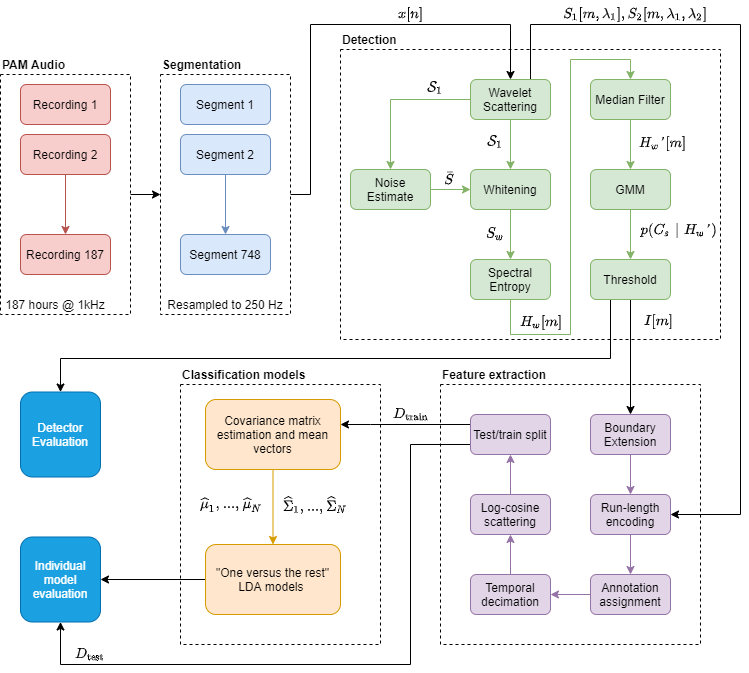
\includegraphics[width=0.9\textwidth]{system_diagram_v2.png}
    \caption{The detection and classifying system. The audio database constists of 1-hour long recordings, which are segmented for computational efficiency. The detection system provides input to the feature extraction and classification steps. The classifier and detector are evaluated separately in this study.}
    \label{fig:system}
\end{figure}

\clearpage

\section{Data}
\label{sec:data}
In this paper, we use an open source dataset recorded over the period of one year in the Casey Islands of Antarctica in 2017, as detailed in \citep{casey2017}. This dataset contains 187 audio files of approximately 1 hour duration each. Recordings took place over the entire year. The hour-long audio recordings are spaced at intervals of approximately 42 hours apart, sampled at 1 kHz. This dataset was chosen instead of the other datasets presented in {\citep{casey2017} due to its reliability, abundance of blue whale annotations and annotation end-point accuracy. Other datasets contained many annotations which were not significantly above the noise level, have inaccurate time localisation regarding the starting and endpoints of the annotation, and/or did not contain enough annotations.

We do not perform any annotation cleaning, as this will unfairly bias our results towards high \ac{snr} detection and classification. However, inaccurate analyst annotations are a significant concern \citep{casey2019}, where some studies discard annotations based on estimated \ac{snr} to improve the ``ground truth" used for accuracy measurements \citep{blue_fin_detection}. Analyst annotation inaccuracies are discussed in greater detail in the later sections of this paper.

For this study, we split each hour-long recording into segments of $2^{18}$ samples after re-sampling to 250 Hz, with the end segment often having less samples. Each segment is approximately 17 minutes in length. Segmentation is performed for memory conservation during computation.

Annotations are provided that give the time-frequency bounding boxes of blue and fin whale vocalisations, among others. In this paper, we mainly focus on the blue whale vocalisations as this is the class with the greatest abundance in this dataset. We also include fin whale vocalisations during detector evaluation. However, due to low \ac{snr} and annotation overlap, very few fin whale samples reach the classification stage. The Casey Islands dataset contains a total of 2988 blue whale annotations, separated as \textit{Bm-A}, \textit{Bm-B}, \textit{Bm-Z} and \textit{Bm-D} types. Figure \ref{fig:Bm_Ex} shows a 1-st level \ac{ws} decomposition ($\mathcal{S}_1$) of high SNR examples of these vocalisation types. Table \ref{tab:numannotations} summarises the number of annotations within this dataset.

\begin{figure}
     \centering
     \begin{subfigure}[]{0.45\textwidth}
         \centering
         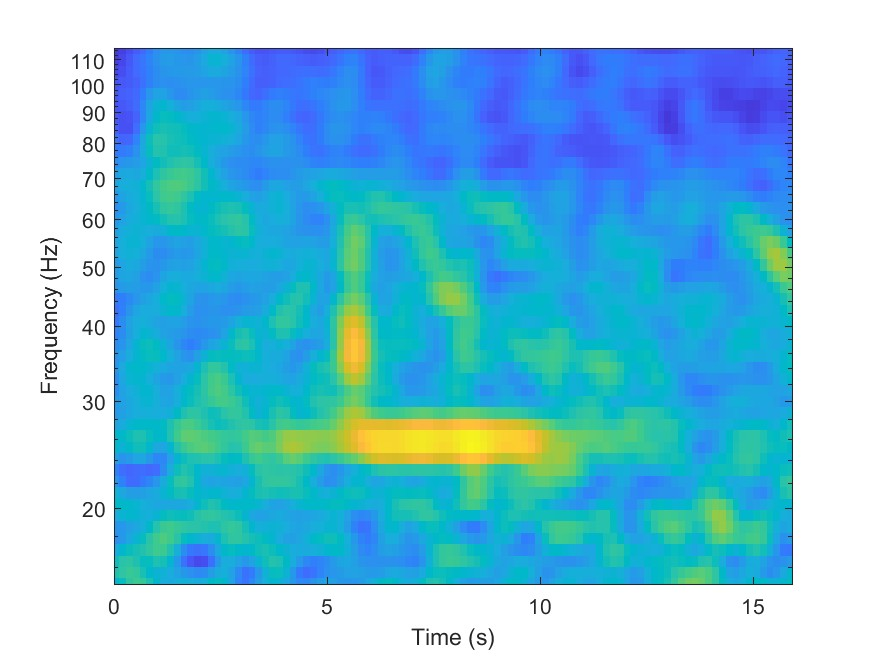
\includegraphics[width=\textwidth]{Bm_Ant-A_11.jpg}
     \end{subfigure}
     \hfill
     \begin{subfigure}[]{0.45\textwidth}
         \centering
         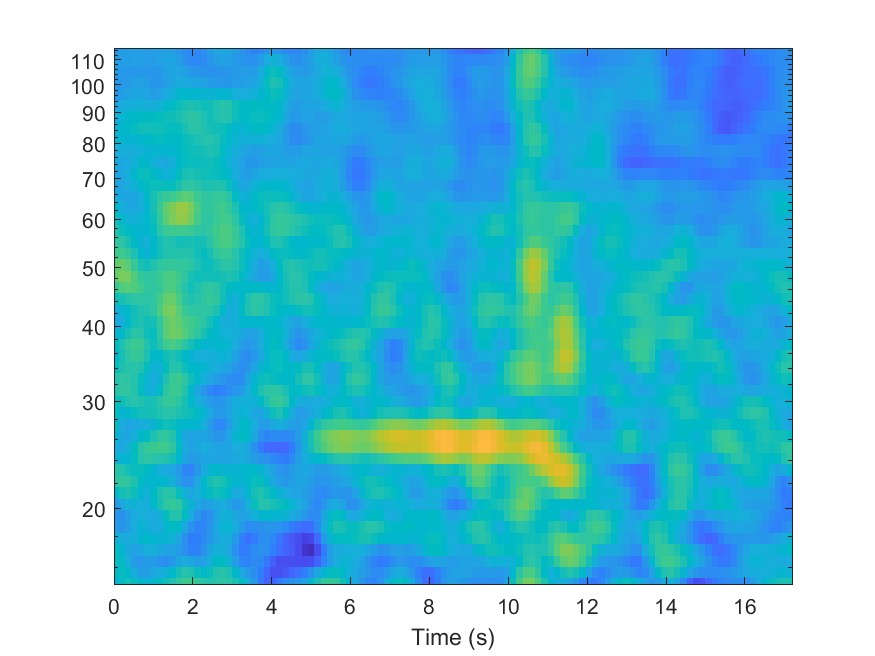
\includegraphics[width=\textwidth]{Bm_Ant-B_54.jpg}
     \end{subfigure}
     \hfill
     \begin{subfigure}[]{0.45\textwidth}
         \centering
         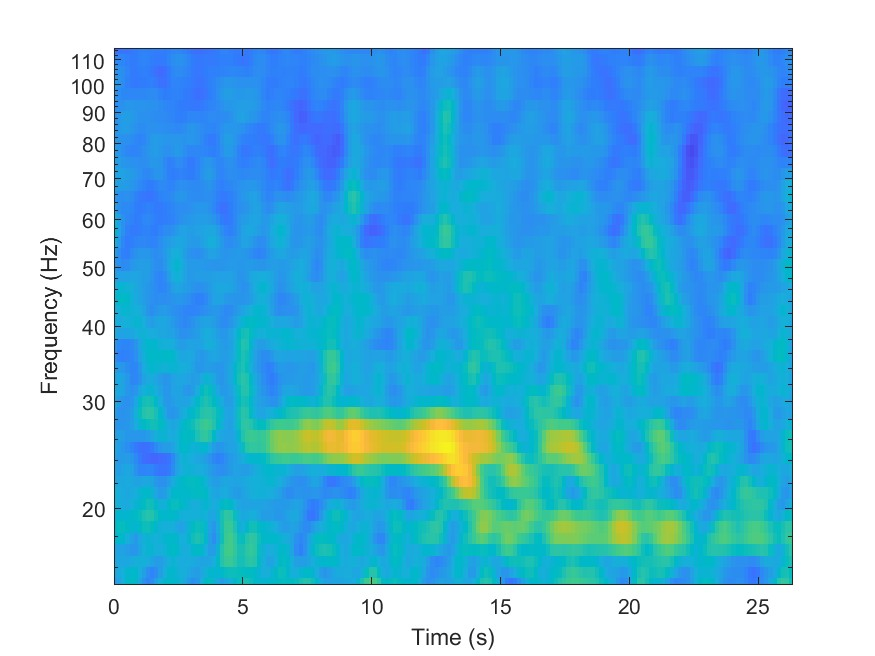
\includegraphics[width=\textwidth]{Bm_Ant-Z_98.jpg}
     \end{subfigure}
     \hfill
     \begin{subfigure}[]{0.45\textwidth}
         \centering
         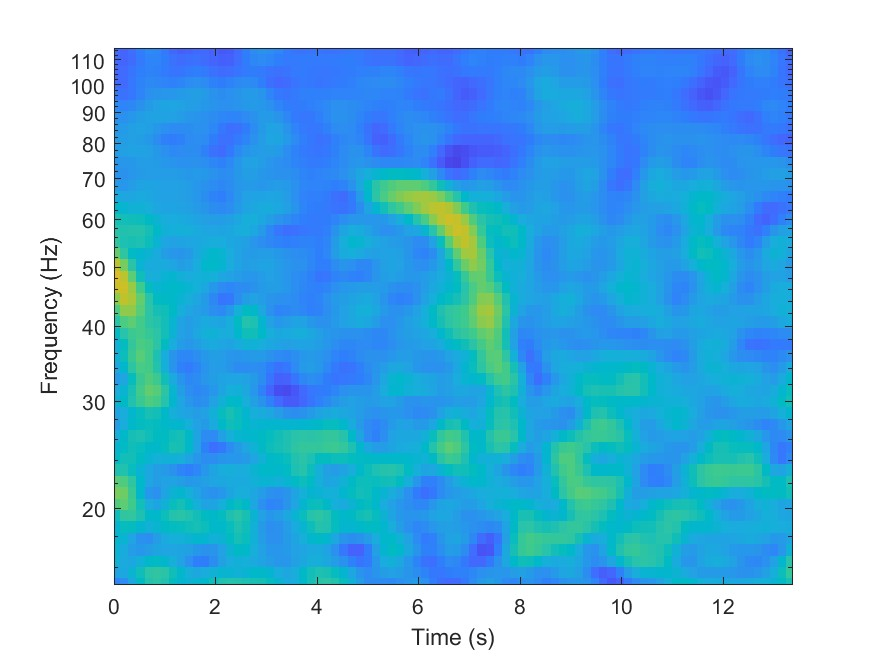
\includegraphics[width=\textwidth]{Bm_D_173.jpg}
     \end{subfigure}
        \caption{High SNR examples of the first level scattering transform to illustrate the characteristics of blue whale calls. Note the logarithmic frequency scale.  \textit{Bm\_Ant\_A} (a) is a constant frequency pulse which occurs around 20 Hz. \textit{Bm\_Ant\_B} (b) and \textit{Bm\_Ant\_Z} (c) are similar to \textit{Bm\_Ant\_A}, but with the addition of frequency modulated tails. \textit{Bm\_D} (d) is a frequency modulated downsweep which typically starts around the 80 Hz and sweeps to 30 Hz.}
        \label{fig:Bm_Ex}
\end{figure}

\begin{table}[h!]
\caption{Total number of annotations in the Casey 2017 dataset.}
\label{tab:numannotations}
% \begin{ruledtabular}  
% \renewcommand{\arraystretch}{0.8}
\begin{tabular}{lrr} 
\textbf{Vocalisation}      & \textbf{Number of annotations} & \textbf{Estimated False positives (\%)} \\ \hline
Bm\_Ant\_A & 1741  & 5 - 10               \\
Bm\_Ant\_B & 558  & 5 - 10                 \\
Bm\_Ant\_Z & 119    & 1 - 2               \\
Bm\_D      & 553     & 8 - 15              \\
Bp\_20Hz & 78        & 1 - 3             \\
Bp\_20Plus & 214     & 1 - 3               \\ 
Total & 3263 & 5 - 10\\ 
\end{tabular}
% \end{ruledtabular}
\end{table}

We estimate the number of false positives by investigating a subset of annotations (at least 100 when possible) and determining which are more probable to be noise than a vocalisation according to their $\mathcal{S}_1$ coefficients as portrayed by Figures \ref{fig:Bm_Ex} and \ref{fig:det_example_1}. This task is difficult to perform with absolute precision, so we provide a lower and upper bound for these estimates such that they are a fair reflection of the uncertainty. The number of missed detections require more investigation and expertise and is out of scope for this study. The false positive proportions are indicated in Table \ref{tab:numannotations}, with the total proportion of false positives calculated by considering the proportion of annotations per class.

\begin{table}[h!]
    \centering
\caption{Estimated erroneous (false positives) proportion of annotations per class that could be considered noise. This table does not reflect on whether annotations are of the correct class (i.e., misclassifications). The total proportion of false positives are calculated according to the number of annotations per class.}
\label{tab:errannotations}
% \begin{ruledtabular}    
\begin{tabular}{lr} 
\textbf{Vocalisation}      & \textbf{False positives (\%)} \\ \hline
Bm\_Ant\_A & 5 - 10                 \\
Bm\_Ant\_B & 5 - 10                  \\
Bm\_Ant\_Z & 1 - 2                  \\
Bm\_D      & 8 - 15                  \\
Bp\_20Hz & 1 - 3                   \\
Bp\_20Plus & 1 - 3                   \\
Total & 5 - 10\\ 
\end{tabular}
% \end{ruledtabular}
\end{table}


\clearpage

\section{Wavelet Scattering}
\subsection{Filter Bank Construction}

This paper utilises a modified version of the wavelet scattering transform, as detailed by \citet{ws}. Given a mother wavelet $\uppsi(t)$ with energy concentrated at 1 rad/s, the wavelet dilated by a factor $\lambda$ is notated by
\begin{equation}
\label{eqn:waveletscaling}
    \uppsi_\lambda(t) = \lambda \uppsi(\lambda t).
\end{equation}

The multiplicative scaling of $\lambda$ ensures that dilation results in constant peak Fourier amplitude in the frequency domain, therefore resulting in L1-normalisation. When $\uppsi$ is centered at 1 rad/s, then $\lambda$ is also the center frequency of the filter (in rad/s) specified by $\uppsi$.

 A typical choice of $\uppsi$, also the choice used in this paper, is the Morlet wavelet, given by
\begin{equation}
\label{eqn:morlet}
    \uppsi(t) = (e^{jt} - \beta) \theta_\sigma(t),
\end{equation}
with $\sigma$ indicating the time support of $\uppsi$ and $j$ is the imaginary unit. The shifting factor $\beta$ ensures that $\uppsi(t)$ satisfies the admissibility criterion (zero-mean). A Gaussian with zero mean and standard deviation $\sigma$ is denoted by $\theta_\sigma(t) = \frac{1}{\sigma\sqrt{2 \pi}} e^{-\frac{1}{2}\left(\frac{t}{\sigma}\right)^2}$, thus resulting in $\beta = \frac{\theta_{1/\sigma}(-1)}{\theta_{1/\sigma}(0)}$.

A filter bank is constructed with $Q$ wavelets per octave. To ensure adequate overlap with adjacent filters, we set $\sigma = Q$. The set of dilation factors $\Lambda$ in the filter bank is constructed with $\lambda_{n+1} = 2^{\frac{1}{Q}} \lambda_n$, where $\lambda_0$ sets the first center frequency in the filter bank, and $\lambda_k \le \omega_\text{max}$ is the last filter specified by the maximum frequency $\omega_\text{max}$.

Discretised filter impulse responses are constructed using
\begin{equation}
    \uppsi_\lambda[n] = \begin{cases}
        \uppsi_\lambda\left(\frac{n}{f_s}\right), \ n \in \{-N, ..., N\} \\
        0, \ \text{otherwise}
    \end{cases} , \ \lambda \in \Lambda.
\end{equation}
$N = \left\lceil\frac{5 Q}{\lambda_0} \right\rceil$ provides an adequate coverage of the lowest-frequency wavelet -- 5 standard deviations of  $\uppsi_{\lambda_0}[n]$.

The operator $\mathcal{U}$ is used to define the scalogram of a discrete signal $x[n]$ sampled at a frequency of $f_s$:
\begin{equation}
    \mathcal{U}x[n, \lambda] = \left|x[n] * \uppsi_\lambda[n]\right|,\  \lambda \in \Lambda.
\end{equation}
The scalogram extracts the band-limited amplitudes of each frequency band in $\Lambda$. Since the modulus operator $|\cdot|$ is effectively amplitude demodulating a band-limited analytic signal, the maximum bandwidth resulting from $\mathcal{U}$ is the bandwidth of $\uppsi_{\lambda_\text{max}}$. We define this bandwidth as 2 standard deviations of $\Psi_{\lambda_\text{max}}(\omega)$, corresponding to $2\frac{\lambda_\text{max}}{Q}$ rad/s. This allows the critical down-sampling of $\mathcal{U}x$ by a factor of $d = \left\lfloor\frac{\pi f_s Q}{2\lambda_\text{max}}\right\rfloor$. We denote the down-sampled scalogram as $\mathcal{U}_{\downarrow d}x$.  %should I downsample by 2 before entering the filterbank??

Additional to the scalogram, a further filtering and decimation step is performed to obtain the scattering coefficients. This is accomplished by utilising a Gaussian low-pass filter $\varphi(t)$ with a user-specified standard deviation of $\frac{T}{2\pi}$ seconds (cutoff frequency of $\frac{1}{T}$ Hz). $T$ is referred to as the invariance scale. The scattering operator $\mathcal{S}$ performs filtering of the scalogram:
\begin{equation}
    \mathcal{S}x[n, \lambda] = \mathcal{U}x[n, \lambda] * \varphi[n], \ \lambda \in \Lambda,
\end{equation}

For computational efficiency, the critically down-sampled scattering coefficients are instead calculated as
\begin{equation}
\label{eqn:scattering:downsample}
    \mathcal{S}_{\downarrow r}x[n, \lambda] = \left(\mathcal{U}_{\downarrow d}x[n, \lambda] * \varphi_{\downarrow d}[n]\right)_{\downarrow r}, \ \lambda \in \Lambda,
\end{equation}
with $r = \left\lfloor\frac{f_s}{ 4 T d V}\right\rfloor$ and $V$ indicating the oversampling factor, since $T$ further band-limits the content when chosen such that it is smaller than the time support of $\uppsi_{\lambda_\text{max}}$.

The discretisation of $\varphi(t)$ is identical to that of $\uppsi_\lambda(t)$. The down-sampling factor $r$ down-samples to within 2 standard deviations of $\Phi(\omega)$, as is done with $\uppsi$. The resulting sampling frequency of the scattering coefficients is approximately $\frac{4}{T}$, which may not be exact due to the compounding down-sampling steps of $r$ and $d$.

To implement the filter bank as defined by $\Lambda$, we use the MATLAB Parallel Processing toolbox, with all convolutions carried out as \ac{fft} convolutions on the \ac{gpu}. We pre-compute the \acp{fft} of the filter bank and the low-pass filter for fast execution, thereby only requiring a \ac{fft} on the input signal. This limits the input signal to a specified length, set to the segment size of $L$. Shorter signals are zero-padded and stripped after convolution.

\subsection{Scattering Transform}
A scattering transform is performed by $F$ scattering filter banks defined by $\{\Lambda_1, ..., \Lambda_F\}$. A scattering transform to the $i$'th level is denoted by the operator $\mathcal{S}_i$. We suppress notation indicating time dependence for clarity. The scattering transform performed on a signal $x$ is given as follows:
\begin{gather} 
    \mathcal{S}_0 x (t) = x * \varphi \\ 
    \mathcal{S}_1 x(t, \lambda_1) = \left|x * \uppsi_{\lambda_1}\right| * \varphi, \ \lambda_1 \in \Lambda_1 \\
    \mathcal{S}_2 x(t, \lambda_1, \lambda_2) = \left|\left|x * \uppsi_{\lambda_1}\right| * \uppsi_{\lambda_2}\right| * \varphi, \ (\lambda_1, \lambda_2) \in \Lambda_1 \times \Lambda_2 \\
    \mathcal{S}_i x(t, \lambda_1, ...,  \lambda_i) = \left|\left|...\left|x * \uppsi_{\lambda_1}\right|*...\right| * \uppsi_{\lambda_i}\right| * \varphi, \ (\lambda_1, ..., \  \lambda_i) \in \Lambda_1 \times ... \times \Lambda_i  \label{eqn:scat2}
\end{gather}

Each scattering filter bank defined by $\Lambda_i$ is constructed by the user. In this paper, we neglect the 0'th level scattering transform $\mathcal{S}_0$ since signals of interest are contained in the 20-120 Hz band, thereby not requiring any low-frequency information. We additionally only utilise up to the second level scattering $\mathcal{S}_2$ for feature extraction. The down-sampling steps detailed by equation (\ref{eqn:scattering:downsample}) are only performed by $\mathcal{S}_1$.



The scattering computations used in this study are given by
\begin{gather}
\label{eqn:scattering:s1}
    \mathcal{S}_{1}x [n, \lambda_1] =  \left(\mathcal{U}_{\downarrow d}x * \varphi_{\downarrow d}\right)_{\downarrow r}, \ \lambda_1 \in \Lambda_1; \\
    \label{eqn:scattering:s2}
    \mathcal{S}_{2}x [n, \lambda_1, \lambda_2] =  \left(\left| \mathcal{U}_{\downarrow d}x * \left(\uppsi_{\lambda_2}\right)_{\downarrow d}\right| * \varphi_{\downarrow d}\right)_{\downarrow r}, \ (\lambda_1, \lambda_2) \in \Lambda_1 \times \Lambda_2.
\end{gather}
Refer to Figure \ref{fig:scattering} for a visualisation of the successive filtering steps to perform a scattering computation.

\begin{figure}[h]
    \centering
    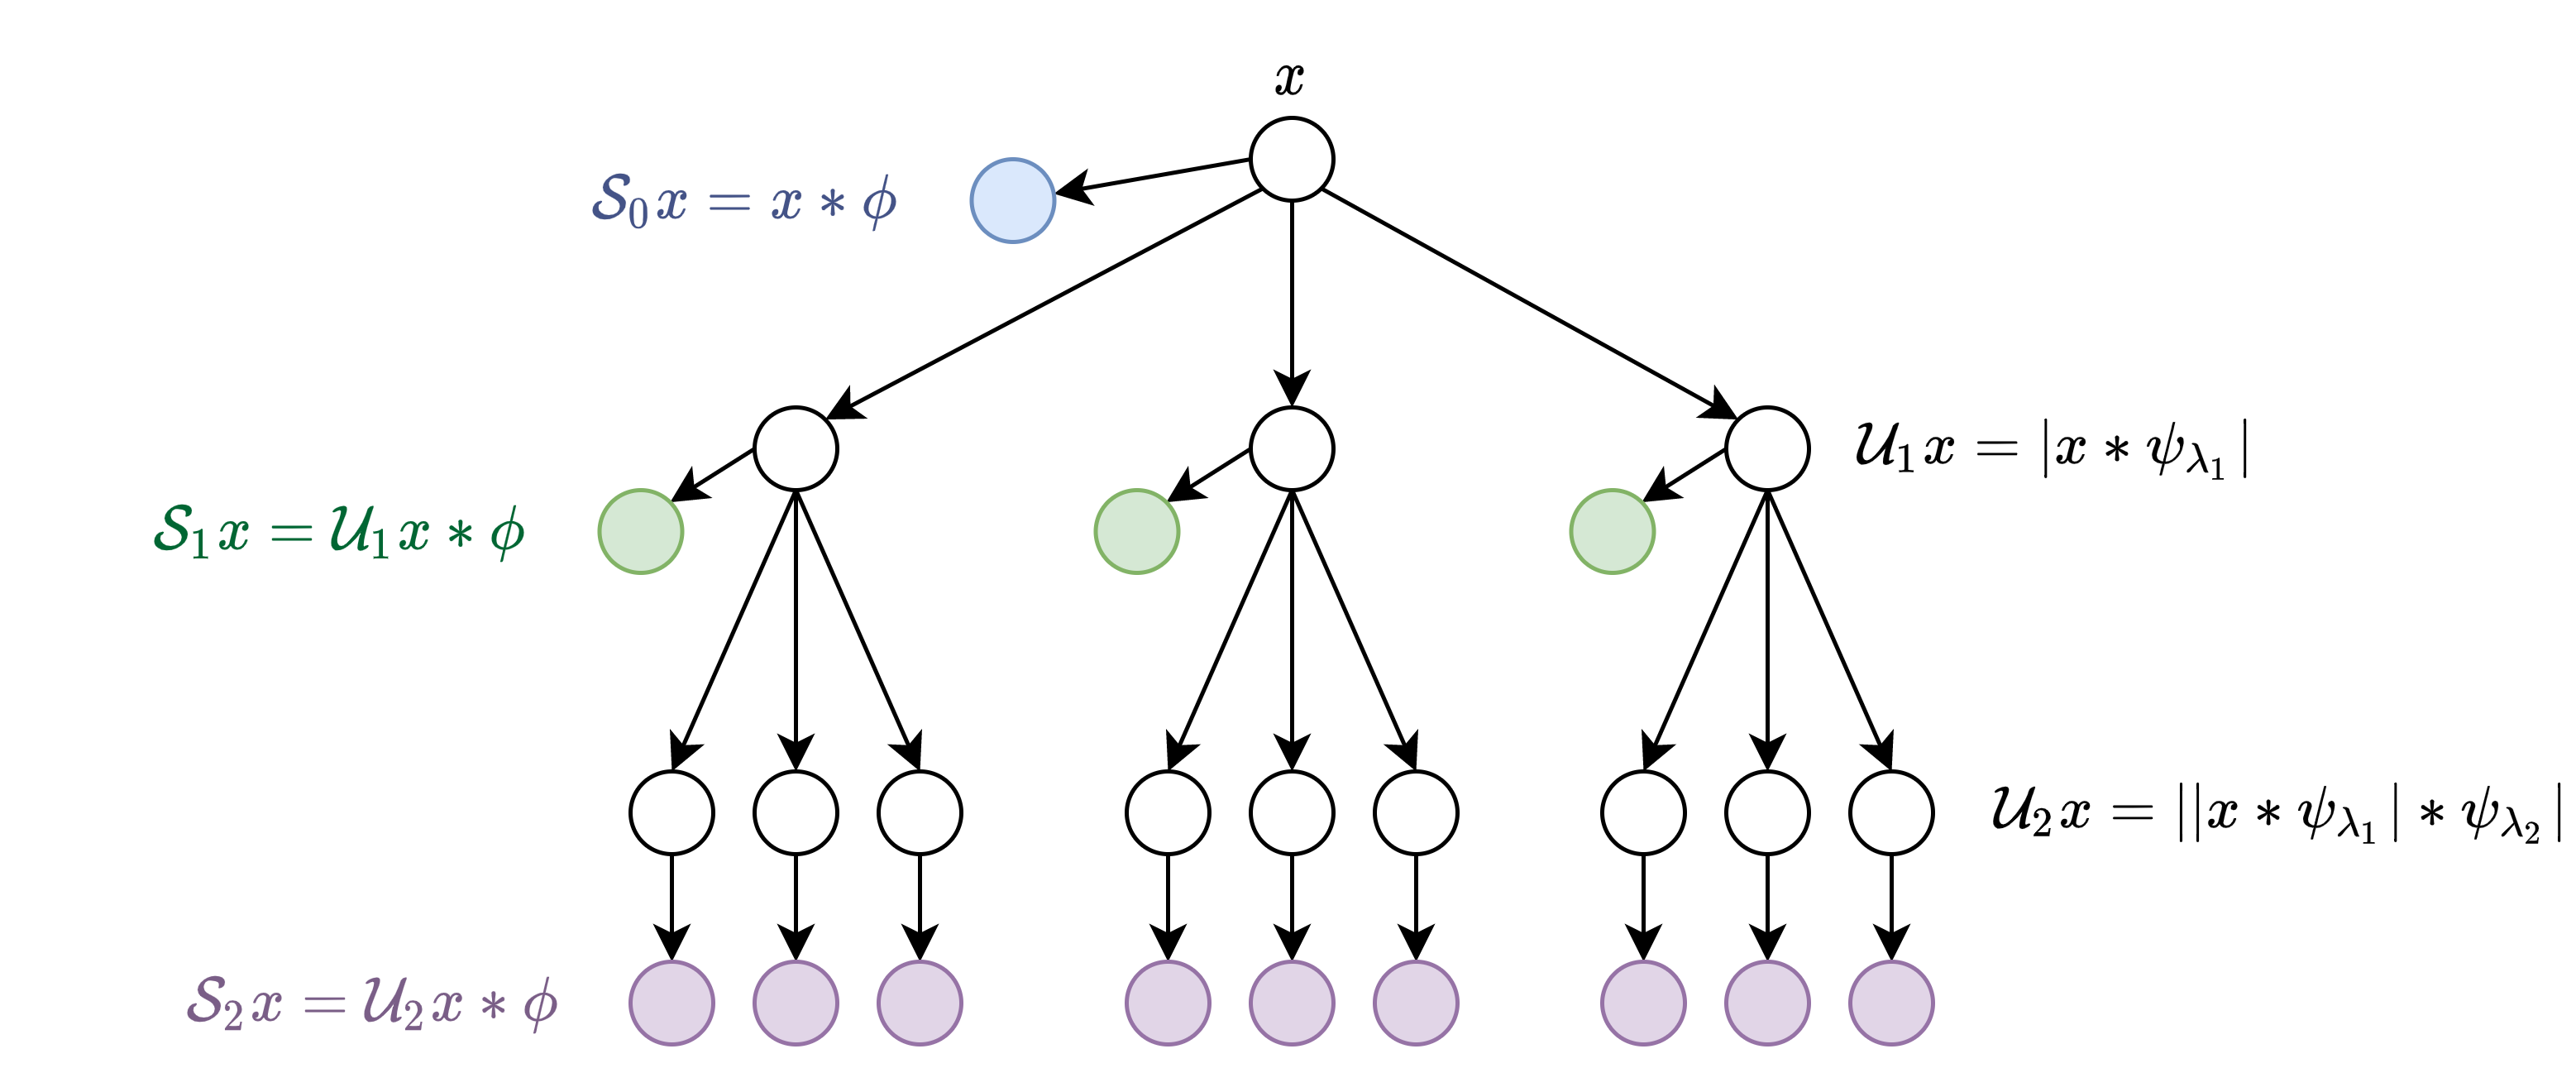
\includegraphics[width=0.9\textwidth]{scattering.png}
    \caption{An illustration of the successive filtering operations performed by a scattering transform. Nodes in colour represent the extracted scattering coefficients, which is down-sampled according to an invariance scale specified by the user.}
    \label{fig:scattering}
\end{figure}

For computational efficiency, it is not required to to calculate all paths for $\lambda_2$, since the lower frequency filters defined by $\Lambda_1$ have small bandwidths, implying their demodulated coefficients may not have energy contained in all the paths defined by $\Lambda_2$. In this study, we only compute the $\mathcal{S}_2$ scattering coefficients when 
\begin{equation}
\label{eqn:restrictlambda2}
    \lambda_2 - \frac{\lambda_2}{Q_2} <  \frac{\lambda_1}{Q_1},
\end{equation}
where $Q_1$ and $Q_2$ are the number of filters per octave for each filter bank defined by $\Lambda_1$ and $\Lambda_2$. A similar optimisation is also performed by \citet{ws_audio}. The filter-banks used in this paper is shown in Figure \ref{fig:fb}.

The second filter banks in equations (\ref{eqn:scattering:s1}, \ref{eqn:scattering:s2}) is sampled at a rate of $f_{ss} = \frac{f_s}{d}$. This implementation differs from the fast computation suggested by \citet{ws_audio}. Typically, lower frequency filters are arranged so that the maximum time support does not exceed the time support of $\varphi$. Therefore, lower frequency filters are linearly spaced, whereas higher frequency filters are exponentially spaced when their time support become smaller than $T$. In the implementation for this paper, all filters are exponentially spaced, regardless of their time support exceeding $\varphi$. The resulting information leakage is largely irrelevant in the classification step for this paper, as later detailed in Section \ref{sec:cls}. For models dependent on time information, such as \acp{hmm} or \ac{lstm} networks, information leakage may affect results and the restriction of the time support of $\uppsi$ specified by \citet{ws_audio} should rather be used.

% In summary, we construct the filter banks using
% \begin{gather}
% \label{eqn:configfb1}
% \Lambda_1 = \left\{\lambda_n \ \middle| \lambda_{n+1} = 2^\frac{1}{Q_1}\lambda_n,\ n \in \mathbb{N}_0,\ \lambda_0 = 2 \pi  f_\text{min},\ \lambda_\text{max} \leq 2 \pi f_\text{max} \right\},\\
% \label{eqn:configfb2}
% \Lambda_2 = \left\{ \lambda_n \ \middle| \lambda_{n+1} = 2^\frac{1}{Q_2}\lambda_n,\ n \in \mathbb{N}_0,\ \lambda_0 = \frac{2\pi}{T},\ \lambda_\text{max} \leq \frac{\sup (\Lambda_1)}{Q_1} \right\}.    
% \end{gather}



\begin{figure}[h]
    \centering
    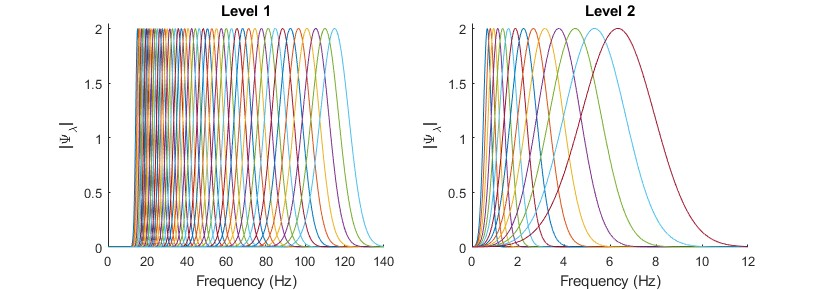
\includegraphics[width=1\textwidth]{fb.jpg}
    \caption{The filter banks used in this study, with $Q_1 = 16$ and $Q_2 = 4$. The filter bank used to calculate $\mathcal{U}_1$ is shown on the left and the $\mathcal{U}_2$ filter bank on the right. Note that the maximum magnitude of 2 accounts for the analytic nature of the wavelet, thereby capturing the true frequency amplitudes in a signal.}
    \label{fig:fb}
\end{figure}

\clearpage
\section{Improved Spectral Entropy Detector}
The \ac{se} detector described by \citet{mypaper} is improved in this section. Rademan shows empirically that the \ac{cwt} yields improved results compared to the \ac{stft} for practical \acp{snr}. As such, we utilise the first level scattering coefficients $\mathcal{S}_{1}$, since it is equivalent to a down sampled version of the \ac{cwt}. We improve on the detector posed by Rademan by introducing true probabilistic output and spectral noise whitening.

\subsection{Spectral Entropy}
\label{sec:spectral_entropy}
Given a discrete-time signal $x[n]$, the first level scattering coefficients are expressed as
\begin{equation*}
	X[k, m] = \mathcal{S}_1x[m, \lambda_k],\ \lambda_k \in \Lambda_1
\end{equation*}
where $k$ is the frequency index and $m$ is sample index. This notation is adopted to emphasise that $X$ is a \ac{tf} decomposition similar to a \ac{stft}.

The power scalogram $S[k, m]$, which is proportional to the equivalent sinusoidal power per frequency band, may be derived from as $S[k,m] = X^2[k, m]$. $S$ is used to construct a time-varying entropy measure $H[m]$, based on Shannon's entropy:
\begin{gather}
\label{eqn:specdist}
	P[k,m] = \frac{S[k,m]}{\sum_{j=0}^{|\Lambda_1|-1} S[j,m]}; \\
\label{eqn:entropy}
	H[m] = - \sum_{k=0}^{|\Lambda_1|-1} P[k,m] \log (P[k,m]).
\end{gather}

% This detector is highly effective under the following assumptions:
% \begin{enumerate}
%     \item  Signals of interest produce scattering coefficients which are sparse in the frequency domain, much larger than noise coefficients. This holds true for periodic and band-limited transient signals. This detector therefore measures the extent of sparsity in the frequency domain over the time invariance scale specified by $T$.
%     \item The noise \ac{psd} is smooth and relatively consistent over the considered time period.
% \end{enumerate}

% Given the aforementioned signal and noise assumptions are true, distinct high and low values in $H[m]$ are created, corresponding to noise and signal respectively.

\subsection{Improving SE Robustness}

Pre-whitening the power spectrum is an effective method of increasing the robustness between signal and noise entropy measures, and serves to stabilize the noise entropy level by enforcing the assumption of stable noise \ac{psd}. To accomplish the whitening, a robust noise \ac{psd} estimator which can function with and without signal presence is required. 

A rolling median filter operator $\text{RM}_v^B$ acting on a signal $y[v, w]$ with respect to the index $v$, is defined as
\begin{equation}
    \text{RM}_v^B y[v, w] = \underset{z}{\text{median}}(y[z,w]), \ z \in \left\{v - \frac{B-1}{2}, ..., v, ..., v + \frac{B-1}{2}\right\},
\end{equation}

\noindent where $B$ is an odd number describing the length of the filtering window. Similarly, we define a rolling average operator $\text{RA}_v^B$ as
\begin{equation}
    \text{RA}_v^B y[v, w] = \frac{1}{B}\sum_z y[z,w], \ z \in \left\{v - \frac{B-1}{2}, ..., v, ..., v + \frac{B-1}{2}\right\}.
\end{equation}

Under the signal and noise assumptions specified in subsection \ref{sec:spectral_entropy}, the coefficients of potential signals are first suppressed by median filtering over the frequency indices $k$, followed by another rolling median estimate over time indices $m$ to suppress any transient signals. Finally, a rolling average calculates the time-varying noise PSD. We utilise the amplitude spectra in this estimation, as we find this works better in practise as squaring increases the noise variance and amplifies outliers.

\begin{equation}
\label{eqn:psdestimate}
    \bar{S}[k, m] = \text{RA}_m^{F} \left( \text{RM}_m^{D} \left(\text{RM}_k^{B} \sqrt{S[k,m]}\right) \right)^2.
\end{equation}
In this paper, we set $B=9$ frequency bins, $D$ to a value corresponding to 5 seconds, and $F$ to 60 seconds. 

% Refer to Figure \ref{fig:noise_estimate_ex} for a visualisation of the robust noise \ac{psd} estimator from equation (\ref{eqn:psdestimate}).

% \begin{figure}[h]
%     \centering
%     \includegraphics[width=0.9\textwidth]{noise_estimation.eps}
%     \caption{An illustration of the noise estimation technique. This example contains varying noise conditions with blue whale calls are shown. The original $\mathcal{S}_1$ coefficients are shown on the left, with the noise estimate on the right. Note how the noise estimation method adequately suppresses tonal and transient signals.}
%     \label{fig:noise_estimate_ex}
% \end{figure}

A whitened power decomposition is calculated:
\begin{equation}
\label{eqn:whitened_scalogram}
    S_w[k,m] = \frac{S[k,m]}{\bar{S}[k, m]}.
\end{equation}
$S_w$ is used instead of $S$ to produce the whitened spectral distribution $P_w$ and \ac{se} $H_w$ with equations (\ref{eqn:specdist}) and (\ref{eqn:entropy}) respectively. As in the related study by \citet{mypaper}, a rolling median filter is used as an effective method to stabilize the \ac{se} measure:
\begin{equation}
    H_w'[m] = \text{RM}_m^{R} (H_w[m]).
\end{equation}

% \subsection{Noise Conditions}
% The noise conditions estimated by equation (\ref{eqn:psdestimate}) are evaluated in this section. The importance of adaptive algorithms is demonstrated by referring to the volatility of the noise in False Bay.

% All power spectrograms in this study are calculated using a Blackman window with 512 samples (256 ms), with 448 samples (224 ms) of overlap. The noise estimate $\bar{S}[k]$ is calculated for each segment with $L = 15$ and $h[k]$ as a Gaussian smoothing filter with a standard deviation of 5 samples. The detector is configured to only consider frequencies above 30 Hz, since this is where all the signals of interest may lie.

% Figure \ref{fig:psdovertime} illustrates how the noise \ac{psd} varies over time. Large variations are present, with the total noise power showing some periodic behaviour over time corresponding to tide, weather and environment changes. Total noise power is calculated by summing over the \ac{psd} estimated for frequencies above 30 Hz. 

% \begin{figure}[h]
%     \centering
%     \includegraphics[width=\textwidth]{psd_over_time.pdf}
%     \caption{The noise conditions over time for the test set. All noise magnitude measurements are normalised according the maximum \ac{psd} observed in the test set. The range of the observed noise vary from 26-60 dB for each of the frequency bins.}
%     \label{fig:psdovertime}
% \end{figure}

\subsection{GMM Automatic Threshold Selection}
\Ac{pam} system recordings which span multiple days are bound to be subjected to many noise conditions when tides, weather and the presence of wildlife change. As such, automatic threshold selection for small audio segments which take into account the specific conditions of the segment is paramount, since a fixed threshold will not necessarily yield good results over the entire database.

In the previous study by \citet{mypaper}, the k-means algorithm \citep{origkmeans} is used to find an adaptive estimate for the low and high levels of an audio segment and generate a pseudo-probabilistic output of signal presence. This pseudo-probability is a first step in normalizing the entropy, but fails to account for the variance of the low and high levels respectively, since the k-means algorithm assumes spherical (equal variance) clusters without accounting for the prior probability of a cluster (i.e., the proportions of signal and noise within the audio segment).

Although this allows for normalized measure between 0 and 1, there is still some uncertainty on the threshold selection, and it requires a hyper-parameter to  ``squeeze" the measures around the equi-probability point (0.5) with a specific steepness.

To improve on threshold selection, this paper models the whitened and median filtered \ac{se} measure $H_w'$ with the probability distribution $p(H_w')$ as a mixture of Gaussians. A \ac{gmm} is fitted using the \ac{em} algorithm. The \ac{gmm} model accounts for each \ac{se} level's variance and the prior probability of each level occurring, assuming independence across all time indices $m$:
\begin{gather}
    H_w' | \mathcal{C} = C_n \sim \mathcal{N}(\mu_n, \sigma_n^2) \\   
    H_w' | \mathcal{C} = C_s \sim \mathcal{N}(\mu_s, \sigma_s^2)
\end{gather}

The observable probability density of $H_w'$ is found through marginalization
\begin{equation}
    p(H_w') = p(C_n)\mathcal{N}(H_w' | \mu_n, \sigma_n^2) + p(C_s)\mathcal{N}(H_w' | \mu_s, \sigma_s^2),
\end{equation}
 where $(\mu_n,\mu_s)$ and $(\sigma_n, \sigma_s)$ are the noise and signal entropy means and variances respectively. $\mathcal{C} \in \{C_n ,C_s\}$ represents the noise and signal levels of $H_w'$. The class prior probabilities $p(\mathcal{C})$ are given by the mixture weights of the \ac{gmm}. The notation $H_w'$ is used to express a random variable, over which all $H_w'[m]$ are independent observations indexed by $m$. The restriction $\mu_n > \mu_s$ is utilised, since the noise entropy measure is always greater than the signal entropy measure under the signal/noise assumptions. 
 
To find the probability of an entropy measure belonging to the signal class $C_s$, Bayes' rule is employed:

\begin{equation}
\label{eqn:entropyposterior}
    p(C_s|H_w') = \frac{p(H_w' | C_s) p(C_s)}{p(H_w')}.
\end{equation}

% Due to $p(C_s|H_w')$ being a true probability measure which accounts for class mean, variance and prior probability, a signal indicator function $\mathcal{I}$ for each entropy measure $H_w'[m]$ is trivially constructed:

% \begin{equation}
% \label{eqn:indicator}
%     \mathcal{I}(H_w'[m]) = \begin{cases}
%     1, & p(C_s|H_w'[m]) \ge p_t \\
%     0, & \text{otherwise}
%     \end{cases}
% \end{equation}

% The threshold value of $p_t$ is indirectly a scaled automatic threshold selection, since the \ac{gmm} parameters automate the shifting and scaling process for each considered audio segment. 

\subsection{Problems with the Posterior}
Equation (\ref{eqn:entropyposterior}) has complex behaviour with respect to its parameters determined by the \ac{gmm}. It is known a priori that a higher entropy corresponds to a larger probability of noise, thus requiring equation (\ref{eqn:entropyposterior}) to be a monotonically decreasing function over the entire observed entropy range of audio segment of interest. To achieve this, \citet{mypaper} uses a sigmoid function which is shaped by the k-means algorithm and a hyper-parameter. Most audio segments from the tested database do not satisfy the condition of monotonocity of the posterior. 

% Refer to Figure \ref{fig:post_problems} for an example of a \ac{gmm} model that does not adhere to these conditions.

% \begin{figure}[h]
%     \centering
%     \includegraphics[width=1\textwidth]{post_problems.eps}
%     \caption{Non-monotonic behaviour of the posterior signal probability as a function of entropy. This example utilises $\mu_n = 4$, $\mu_s = 3$, $\sigma_n = 0.3$, $\sigma_s = 0.7$, $p(\mathcal{C}_n) = 0.6$. Probability densities are shown on the left and the posterior function is shown on the right. Clamping is illustrated with the dashed line on the right.}
%     \label{fig:post_problems}
% \end{figure}

% \begin{figure}[h]
%      \centering
%      \begin{subfigure}{0.45\textwidth}
%          \centering
%          \includegravarphics[width=\textwidth]{det_example.pdf}
%          \caption{Detection using the modified posterior. }
%          \label{fig:det_ex}
%      \end{subfigure}
%      %
%      \begin{subfigure}{0.45\textwidth}
%          \centering
%          \includegravarphics[width=\textwidth]{post_example.pdf}
%          \caption{The unmodified posterior function.}
%          \label{fig:post_ex}
%     \end{subfigure}
%     \caption{An example illustrating the proposed detector output with whitening and posterior modification and it's corresponding non-monotic posterior function when left unmodified. The spectrogram shown (\ref{fig:det_ex}) is suspected to portray fish, which ``hum" at a near-constant frequency and power at irregular intervals for long periods of time. The humming is accurately identified as a signal with high probability by the detector, despite the poor average estimated \ac{snr} of 7 dB (calculated above 100 Hz to neglect anchor rumble in the estimation). The detector also detects anchor rumble since it presents as narrow-band noise. Note that only half of the audio segment is shown in this example. The unmodified posterior function (\ref{fig:post_ex}) in this example clearly illustrates the non-monotonic behaviour, even within the range of the observed entropy levels (shown as the dotted lines). The signal (blue) and noise (orange) Gaussian range estimates in \ref{fig:post_ex} are shown to visualize the width of the distributions. The width of the signal class crosses over the noise class, which presents the need to modify the posterior function with clamping at the turning point.}
%      \label{fig:post^problems} 
% \end{figure}

This paper proposes that the posterior is clamped after reaching the monotonicity limits. Refer to appendix \ref{app:mono} for the derivation of these limits. With this modification made, it is guaranteed that the posterior is a piece-wise function which is either decreasing or remains constant.

\begin{equation}
p_{\text{clamp}}(C_s | H_w') = 
    \begin{cases}
        p_\text{max},&  \sigma_s^2 > \sigma_n^2 \ \wedge \  x < \theta \\
        p_\text{min},& \sigma_s^2 < \sigma_n^2 \ \wedge \ x > \theta\\
        p(C_s | H_w'),&  \text{otherwise}
    \end{cases},
\end{equation}
where
\begin{equation}
    \theta = \frac{\sigma_s^2\mu_n - \sigma_n^2\mu_s}{\sigma_s^2 - \sigma_n^2},
\end{equation}
with $p_\text{max}$ and $p_\text{min}$ as the maximum and minimum values of the posterior function that is observed within the range of $H_w'$.
% \begin{gather}
%     p_\text{max} = \underset{m}{\max} \ p(C_s | H_w'[m]); \\
%     p_\text{min} = \underset{m}{\min} \ p(C_s | H_w'[m]).
% \end{gather}
$p_\text{max}$ and $p_\text{min}$ are numerically approximated\footnote{The maximum and minimum entropy values in the posterior distribution is calculated by sampling 1000 regularly spaced points in the observed entropy range and finding the maximum and minimum of the sampling points. For a more efficient approach, Newton's method may be used.}. For an example of the output of the entropy detector, refer to Figure \ref{fig:det_example_1}. 

\begin{figure}[]
    \centering
    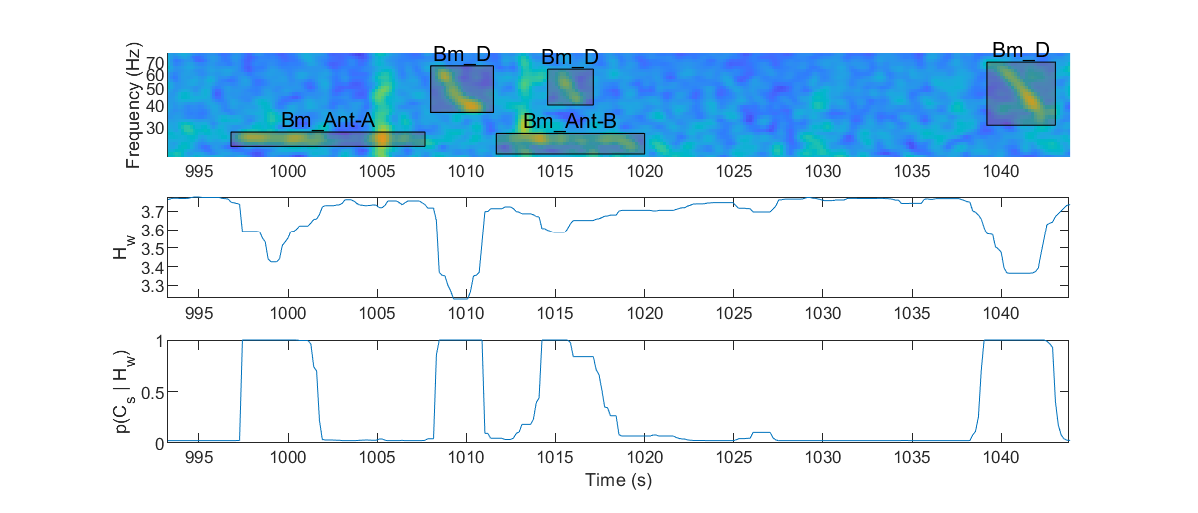
\includegraphics[width=1\textwidth]{detector_example_2.eps}
    \caption{An example of the output of the detector taken from a densely populated vocalisation region of the dataset. The annotation bounding boxes are also indicated (top). In this example, the detector successfully detects all vocalisations. The whitened SE measure is shown (middle) with the posterior probability of signal (bottom).}
    \label{fig:det_example_1}
\end{figure}

% \begin{figure}[]
%     \centering
%     \includegraphics[width=1\textwidth]{detector_example_1.eps}
%     \caption{An example of the output of the detector similar to that of Figure \ref{fig:det_example_1}. Note how the detector also detects two possible low-SNR blue whale vocalisations (not in the annotated dataset) around $t = 95$ and $t = 120$ seconds. The detector cannot distinguish between vocalisation and noise segments fulfilling the detection criteria of $\mathcal{S}_1$ coefficient sparsity. This example section does not contain any annotations, indicating missed annotations by the analyst.}
%     \label{fig:det_example_2}
% \end{figure}



% \clearpage
% \section{Noise}
% \label{sec:noise}
% This section aims to illustrate the variability of noise conditions present in the dataset. We utilise 1-st level \ac{ws} to calculate the noise \ac{psd} over the 15-120 Hz frequency range. Given the noise estimate $\bar{S}$ specified in equation (\ref{eqn:psdestimate}), we convert the L1 normalised scattering coefficients to L2 normalised, thereby preserving the magnitude of energy contained in the filter:

% \begin{equation}
% \label{eqn:psd}
%     \text{PSD}_\text{dB}[k, m] = 20 \log_{10}\frac{\bar{S}[k, m]}{\lambda_k},\ \lambda_k \in \Lambda_1.
% \end{equation}

% For each segment, we calculate the mean and standard deviation to illustrate the noise profile and its withinW-segment variation:
% \begin{gather}
%     \mu_\text{dB}[k] = \frac{1}{M} \sum_m \text{PSD}_\text{dB}[k, m]; \\
%     \sigma_\text{dB}[k] = \frac{1}{M} \sum_m \left(\text{PSD}_\text{dB}[k, m] - \mu_\text{dB}[k]\right)^2.
% \end{gather}

% \begin{figure}[h]
%      \centering
%      \begin{subfigure}[]{0.45\textwidth}
%          \centering
%          \includegraphics[width=\textwidth]{noise_over_time.eps}
%          \caption{Normalised noise power over time.}
%          \label{fig:noise_time}
%      \end{subfigure}
%      \hfill
%      \begin{subfigure}[]{0.45\textwidth}
%          \centering
%          \includegraphics[width=\textwidth]{noise_std.eps}
%          \caption{Standard deviation of the noise estimate within each segment.}
%          \label{fig:noise_std}
%      \end{subfigure}
%      \hfill
%      \begin{subfigure}[]{0.38\textwidth}
%          \centering
%          \includegraphics[width=\textwidth]{noise_average_profile.eps}
%          \caption{The average noise profile and its maximum and minimum bounds within the dataset.}
%          \label{fig:noise_profile}
%      \end{subfigure}
%      \caption{The noise estimates of each segment for the entire dataset. Note that the ridges in (a) are a result of the non-continuous nature of the recordings of this dataset as detailed in section \ref{sec:data}. Some segments contain large noise variations, as seen in (b). The average and range of the noise profile for the entire dataset is seen in (c).}
%      \label{fig:noise}
% \end{figure}

% Refer to Figure \ref{fig:noise} for an illustration of the noise profile over the recorded segments. A large variation in noise power is observed, with low frequency noise power changing by up to 60 dB over the year-long time period. As such, any deployed detector must be adaptive to these conditions, since a non-adaptive threshold will fail for many segments. The method proposed in this paper indirectly incorporates an adaptive threshold using a \ac{gmm} fit to the \ac{se} measure.

% Segments with large noise variation in low frequencies may also indicate blue/fin whale choruses, which are the layered sounds of many whales vocalising at once \citep{casey2017}. Annotations in these sections are likely not very accurate, as the entire audio segment contains vocalisations.

\subsection{Method}

We measure the performance of the detectors via \ac{roc} curves, by testing each annotated sample in the power scalogram $S$. No annotation cleaning is performed and all audio files are included. Annotations which have bounding boxes that do not intersect with the 15-120 Hz band are neglected, since the detectors do not operate outside this bandwidth.

Three \ac{se} detectors are evaluated: \ac{gmm} fitted on the non-whitened $\mathcal{S}_1$ coefficients; \ac{gmm} on the whitened $\mathcal{S}_1$ coefficients; and k-means fitted on the non-whitened $\mathcal{S}_1$ coefficients as performed by \citet{mypaper}. Comparing these detectors will validate that modelling the entropy with a \ac{gmm} and applying whitening yields incremental improvements from the original k-means implementation. As a baseline, we also compare the results to a \ac{bled} which sums over the whitened $\mathcal{S}_1$ coefficients. This form of \ac{bled} is more akin to the detector implementations present in \ac{pam} software, as it indirectly adapts to noise conditions during the whitening process. The whitened \ac{bled} additionally has its energy median filtered in the same manner as the \ac{se} detectors, such that a fair comparison is obtained with respect to whitening and filtering.

To perform unmodified energy detection with wavelet scattering, the average energy $E$ of each time slice calculated using
\begin{equation}
\label{eqn:bled_power}
    E[m] = \frac{1}{\left| \Lambda_1 \right|}\sum_{\lambda_1 \in \Lambda_1} \left(\frac{\mathcal{S}_1 x [m, \lambda_1]}{\sqrt{\lambda_1}}\right)^2,
\end{equation}
which converts the wavelet L1 normalisation from Equation (\ref{eqn:waveletscaling}) to L2. 

Two methods of evaluation are employed. We perform a sample-by-sample evaluation to produce a \ac{roc} curve. This method will measure the proportion of samples which has been detected and therefore penalise sporadic detections. However, this is not an optimal method of measuring the detector. The dataset does not contain accurate annotation bounding boxes, thereby unfairly penalising the detectors based on annotation endpoint accuracy. Additionally, we count the proportion of annotated calls that have at least 1 detected time sample, and plot it against the proportion of noise/un-annotated samples which have been detected. The true efficacy of the detection is therefore determined, however, sporadic detections are not penalised.




\subsection{Results}
\label{sec:detector_results}

Figure \ref{fig:det_roc} shows the \ac{roc} curve for detection on a sample-by-sample basis. Incremental performance improvement is demonstrated by adding a \ac{gmm} and enhancing the detector with whitening. In Figure \ref{fig:det_calls}, we show that the proposed detector is able to detect the majority calls while detecting fewer noise.  As illustrated in many previous studies, \ac{se} greatly outperforms a traditional \ac{bled} detector \citep{entropyJASA}. Whitening is also shown to greatly improve the capabilities of the \ac{bled} detector.

% \begin{figure}[h]
%     \centering
%     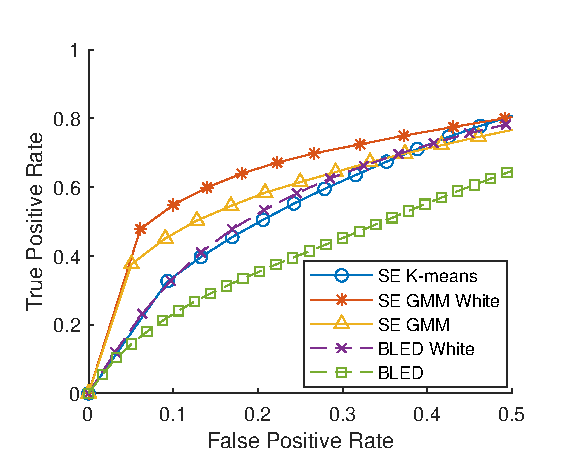
\includegraphics[width=0.6\textwidth]{roc.eps}
%     \caption{The performance of the detectors when compared on a sample-by-sample bases. \ac{se} detectors are indicated as a solid line, while \ac{bled} is dashed. The whitened and median filtered \ac{bled} performs similarly to the k-means \ac{se} detector (unwhitened), but is ouperformed by the whitened \ac{gmm} \ac{se} detector. Adding a \ac{gmm} without whitening indicates incremental improvement over using k-means. }
%     \label{fig:det_roc}
% \end{figure}


% % \begin{figure}[h]
% %     \centering
% %     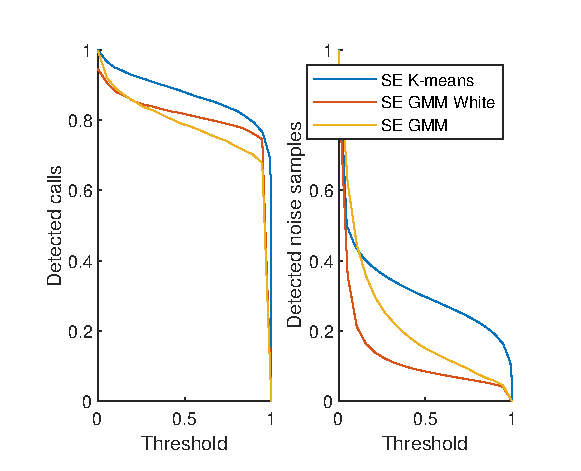
\includegraphics[width=0.6\textwidth]{threshold.eps}
% %     \caption{The proportion of detected blue and fin whale calls and noise samples as a function of the selected probability threshold.}
% %     \label{fig:det_thresh}
% % \end{figure}

% \begin{figure}[h]
%     \centering
%     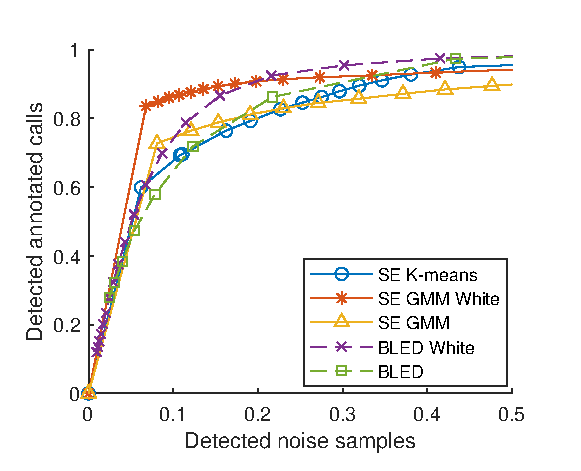
\includegraphics[width=0.6\textwidth]{calls.eps}
%     \caption{The performance curve of the detectors expressed as the percentage of detected noise samples versus the percentage of detected calls. \ac{se} detectors are indicated as a solid line, while \ac{bled} is dashed. The whitened \ac{se} with \ac{gmm} detector significantly outperforms all other detectors.}
%     \label{fig:det_calls}
% \end{figure}

\begin{figure}[h]
     \centering
     \begin{subfigure}[t]{0.45\textwidth}
    \centering
    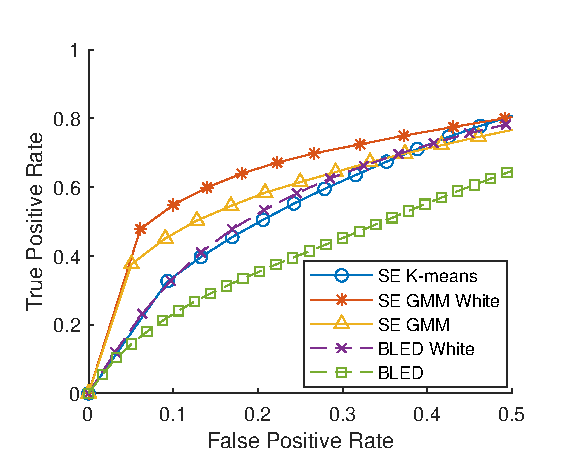
\includegraphics[width=1\textwidth]{roc.eps}    
     \caption{} \label{fig:det_roc}
     \end{subfigure}
     % \hfill
     \begin{subfigure}[t]{0.45\textwidth}
    \centering
    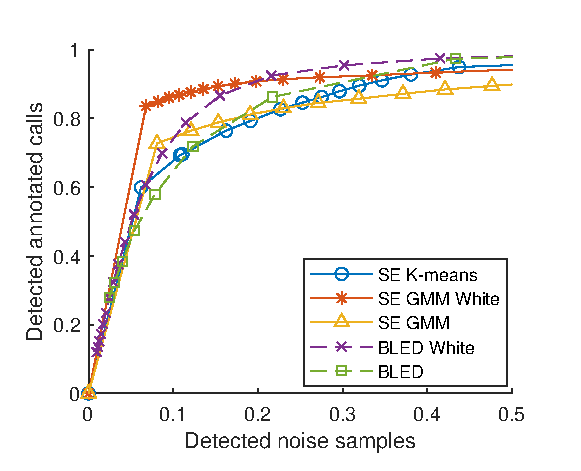
\includegraphics[width=1\textwidth]{calls.eps}    
    \caption{} \label{fig:det_calls}
     \end{subfigure}
     \caption{Results of the evaluated detectors. \ac{se} detectors are indicated as a solid line, while \ac{bled} is dashed. (a) The performance of the detectors when compared on a sample-by-sample bases. (b) The performance curve of the detectors expressed as the percentage of detected noise samples versus the percentage of detected calls. The whitened \ac{se} with \ac{gmm} detector significantly outperforms all other detectors.}
\end{figure}


\begin{table}[h] 
    \centering
\caption{The number of missed calls as a result of a non-converging \ac{gmm} fit.}
\label{tab:convergence}
\begin{tabular}{lc} 
\hline
\textbf{Vocalisation}       & \textbf{Missed vocalisations}  \\ \hline
SE GMM                      & 196 (5.8\%)                      \\
Whitened SE GMM             & 43 (1.2\%)                    \\ \hline
\end{tabular}
\end{table}





\subsection{Discussion}

Results for \ac{stft}-based \ac{bled} has been reported for the Casey Islands 2017 dataset in \citep{casey2017} using the PAMGuard Ishmael energy sum detector. These results are not directly comparable to this paper, since the detectors have additional parameters controlling false positives, such as time length and distance between detections and adaptive thresholding. These detections are measured on a per run-length basis, i.e., over the total run of the detector exceeding a threshold, instead of a per-sample basis. Therefore, this form of measurement may not accurately represent endpoint detection capabilities. 

As seen in Figures \ref{fig:det_roc} and \ref{fig:det_calls}, the proposed \ac{se} detector outperforms the previous method \citep{mypaper}. Typical \ac{bled} with a fixed threshold performs very poorly due to varying noise conditions. \ac{bled} has repeatedly been shown to not be a reliable \ac{poi} detector \citep{internalsignaldetection, entropyJASA}. 

Interestingly, adding whitening to \ac{bled} results in similar performance to the method proposed by \citet{mypaper}. Spectral whitening and \ac{gmm} fitting shows incremental improvements to the k-means based \ac{se} detector. The final proposed detector outperforms the other detectors both in terms of endpoint accuracy (figure \ref{fig:det_roc}) and the number of calls versus noise detected (figure \ref{fig:det_calls}). This paper later discusses the implication of annotation inaccuracies in section \ref{sec:classification_discussion}. As such, the indicated results may not be entirely accurate, and could be better than indicated. From the false positives estimated in Table \ref{tab:numannotations}, all of the detectors likely detect 5-10\% more calls for realistic thresholds than indicated.

\clearpage
\section{Classification}
\label{sec:cls}
We combine the output of the \ac{se} detector with \ac{ws} features and utilise \ac{lda} to classify the detected calls. Our method shares many similarities with studies that also employ \ac{ws} without a \ac{nn}, but differs in allowing for variable window sizes produced by a detector \citep{ws_audio, ws_ecg}.

\subsection{Feature Extraction}
Detections are performed with a posterior signal probability threshold of 0.3, thereby corresponding to 91\% of vocalisations detected, with a significant number of unlabeled noise detections. Refer to Table \ref{tab:numdetections} for the number of detected calls. 

After detection with with a whitened \ac{se} \ac{gmm} detector, we threshold the posterior probability given by Equation (\ref{eqn:entropyposterior}). We ensure that an entire vocalisation is captured by applying a rolling maximum filter over Equation (\ref{eqn:entropyposterior}), thereby extending the boundaries of the detections with a length of $G$. We set the filter length to 6 seconds, thus extending detections by 3 seconds on either side. Note that boundary extension may add additional calls to the detected vocalisations compared to the results from section \ref{sec:spectral_entropy}.

Labels are obtained by assigning each extended detection to an annotation that which occurs in the same timeframe, with the noise class being assigned if there are no corresponding annotations. Annotations have their endpoints shrunk by 5\% to account for endpoint inaccuracies. Detections having multiple annotation assignments which do not belong to the same class are discarded in this study. Noise detections may erroneously overlap with annotations, which could negatively impact the classification results. This is not addressed in this paper.

We dispose of the time dimension across scattering features for each detection by taking the maximum over the consecutive detected indices given by the set $\mathcal{M}$ and normalising power:
\begin{gather}
    \label{eqn:norm_rms}
    \bar{P} = \frac{1}{\left| \mathcal{M} \right|}\sum_{m \in \mathcal{M}} \sum_{\lambda_1 \in \Lambda_1} \left(\frac{\mathcal{S}_1[m, \lambda_1]}{\sqrt{\lambda_1}}\right)^2; \\
    \label{eqn:scatf1}
    f_1[\lambda_1] = \frac{1}{\bar{P}}\underset{{m \in \mathcal{M}}}{\text{max}}\mathcal{S}_1[m, \lambda_1]; \\
    \label{eqn:scatf2}
    f_2[\lambda_1, \lambda_2] = \frac{1}{\bar{P}}\underset{{m \in \mathcal{M}}}{\text{max}} \mathcal{S}_2[m, \lambda_1, \lambda_2].    
\end{gather}
Equation (\ref{eqn:norm_rms}) is the average power over detection indices which is calculated using equation (\ref{eqn:bled_power}).

\Ac{cls} features are used, as detailed by \citet{ws_audio}. First-level \ac{cls} features are directly comparable to \ac{mfcc}, with the addition of the the second level scattering features. The transform is applied to equations (\ref{eqn:scatf1}) and (\ref{eqn:scatf2}) as follows:
\begin{gather}
    F_1[\lambda_1] = \text{DCT}_{\lambda_1}\left(\log f_1[\lambda_1]\right); \\
    F_2[\lambda_1, \lambda_2] = \text{DCT}_{\lambda_2}\left(\log f_2[\lambda_1, \lambda_2]\right),    
\end{gather}
where $\text{DCT}_{x}$ denotes the discreet cosine transform over the variable $x$. The feature vector $v$ is constructed using using $F_1$ and $F_2$ over all significant scattering paths. This dataset is normalised to zero-mean and unit variance.

% The feature vector $v$ is constructed using
% \begin{equation}
%     v = \begin{pmatrix}
%         F_1[\lambda_{11}] \\
%         F_1[\lambda_{12}] \\
%         \vdots \\
%         F_2[\lambda_{11}, \lambda_{21}] \\
%         \vdots \\
%         F_2[\lambda_{1A}, \lambda_{2B}] \\
%         L
%     \end{pmatrix}, \ \lambda_{1a} \in \Lambda_1, \ \lambda_{1b} \in \Lambda_2.
% \end{equation}
% Note that for each $(\lambda_1, \lambda_2)$, the number of coefficients of $\lambda_{2}$ is a function of $\lambda_{1}$ as per the restriction given by equation (\ref{eqn:restrictlambda2}). Finally, all the features are normalised over the entire dataset by subtracting the means of each feature and dividing by each feature's standard deviation.



\subsection{Linear Disciminant Analysis}
We train a multiple ``one versus the rest" \ac{lda} classifiers using a balanced covariance estimate. There are 2 classes (vocalisation and noise) indexed by $i \in \{1, 2\}$, each with $K_i$ training observations. Each model considers only a single vocalisation class and regards all the other classes as noise.  

Due to the similarity between calls of the \textit{Bm\_Ant} classes, models for these classes should not be penalised for misclassifying other \textit{Bm\_Ant} call types. As such, \textit{Bm\_Ant} models have all similar classes removed from their training and test sets. Many fin whale calls do not reach the classification stage of this paper due to their presence in the chorus sections of the audio and overlap. As such, we combine the fin whale vocalisation classes (\textit{Bp\_20Hz}, \textit{Bp\_20Plus}) into a single class (\textit{Bp}) due to their similarity.

We utilise regularised \ac{lda} with prior class probabilities $p(\mathcal{C})$. \ac{lda} assumes that each class is normally distributed, with a single class covariance matrix $\Sigma_\gamma = (1-\gamma)\hat{\Sigma} + \gamma \text{diag}\left(\hat{\Sigma}\right)$, where $\hat{\Sigma}$ is the sample covariance estimate shared between the classes and $\gamma$ is the covariance regularisation hyperparameter. Given an observation $x$ as a column vector, the log posterior probability of $x$ belonging to class $\mathcal{C}_i$ is
\begin{equation}
    \log p\left(\mathcal{C} = \mathcal{C}_i \middle| x\right) = -\frac{1}{2}\Sigma_\gamma^{-1}\hat{\mu}_i x -\frac{1}{2} \hat{\mu}_i^T\Sigma_\gamma^{-1}\hat{\mu}_i + \log p(\mathcal{C}_i) + \beta,
\end{equation}
where $\beta$ is a normalising constant that may be neglected to assign scores to each class.

To combat class imbalance, we use the following estimates:
\begin{gather}
    \label{eqn:lda_median}
    \hat{\mu}_i = \frac{1}{K_i}\sum_{n \in \mathcal{N}_i} x_n ;\\
    \hat{\Sigma}_i = \frac{1}{K_i}\sum_{n \in \mathcal{N}_i} \left(x - \hat{\mu}_i\right)^T\left(x - \hat{\mu}_i\right);\\
    \label{eqn:lda_sigma}
    \hat{\Sigma} = \frac{1}{2}\left(\hat{\Sigma}_1 + \hat{\Sigma}_2 \right),
\end{gather}
where $\mathcal{N}_i$ is the set containing the indices of $x_n$ belonging to class $\mathcal{C}_i$. Equation (\ref{eqn:lda_sigma}) approximates the covariance by assuming equal class weights, although this is typically weighted by the observation proportion in other applications. Equal weighting in shared covariance estimation ensures that all classes are able to significantly contribute to the covariance estimate, which combats the high proportion of noise samples in this study.

The prior probabilities $p(\mathcal{C})$ are typically empirically estimated from the training data. In this study, we employ the following model for prior probabilities to combat the high number of noise observations:
\begin{equation}
    p(\mathcal{C}) = \begin{cases}
        \alpha, \ \mathcal{C} = \mathcal{C}_\text{noise}\\
        1-\alpha,\ \mathcal{C} = \mathcal{C}_\text{vocalisation}
    \end{cases}.
\end{equation}
The hyperparameter $\alpha \in (0,1)$ sets the sensitivity of the classifier to noise detections.



\subsection{Results}
To evaluate our model, we split the training data into training and test sets proportional to the number of items belonging to that class. To demonstrate the practicality of our proposed technique, we perform experiments for different train-test splits with chi-square feature selection. An 80\%-20\% train-test split without feature selection is also used as a baseline. Results are shown in Table \ref{tab:clsres}. Feature selection is performed with a chi-square test of independence (noise versus signal classes). We select features with a statistical significance greater than 0.05, by binning each feature into 10 uniform bins. Feature selection is performed using only the training data.
% \begin{enumerate}
%     \item Training data is composed of 80\% of the noise and signal classes. This experiment illustrates the effectiveness of the the classifier with a full training set. Refer to Table \ref{tab:res80} for the results.
%     \item In practise, large annotated \ac{pam} datasets are not readily available. The second experiment utilises 20\% of the noise and signal classes for training the models. This experiment illustrates the effectiveness of the proposed technique for small datasets, allowing it to be more useful for practical applications.
%     \item Each class, especially the \textit{Bm\_Ant} classes, are bandlimited and may only require specific $\mathcal{S}_2$ features for classification. As such, it may be useful to perform feature selection for each class. For this experiment, we perform a chi-square test of independence and select only features with a statistical significance greater than 0.05, by binning each feature into 10 uniform bins. Feature reduction is only performed using the training data. As a baseline, we again use an 80\%-split for the training data.
%     \item To compare feature selection with the full feature set with little data, we employ another 20\% split with chi-square feature selection.
%     \item Finally, to show that adequate results may still be obtained with very little data, we use a 5\% split combined with chi-square feature selection. 
%     \item We evaluate the classes as is done in the previous experiment, with the 5\% of the lowest SNR calls are removed. SNR is determined by evaluating the power from the detector-provided window and comparing it to the noise power from the noise estimate. This shows that low-SNR and erroneous/partial detections have a significant impact on classification accuracy. Most fin whale calls are discarded due to low SNR, making it impractical to evaluate under the 5/95\% train-test split. As such, this experiment only evaluates blue whale calls.
% \end{enumerate}

Classification accuracy is measured using the observations not included in the test set. Unless specified otherwise, training is repeated 20 times and the results presented are the average accuracy and its standard deviation. We additionally perform a coarse grid search to optimise the hyperparameters $\alpha$ and $\gamma$ and present the results for the best hyperparameters. Hyperparameters are optimised by maximising the cost function $A_\text{Vocalisation} + 2A_\text{Noise}$, with $A$ the accuracy of the test set, thereby enforcing a stricter policy on false detections.




\begin{table}[h!]
\caption{Number of labeled detections for all vocalisations of interest. The detections are produced by the whitened \ac{gmm} \ac{se} detector. A significant number of detections are discarded in the training data due to overlapping.}
\label{tab:numdetections}
% \begin{ruledtabular}
% \renewcommand{\arraystretch}{0.8}
\begin{tabular}{lc} 
\textbf{Vocalisation}      & \textbf{Number of detections}  \\ \hline
Bm\_Ant\_A & 1514              \\
Bm\_Ant\_B & 474              \\
Bm\_Ant\_Z & 91               \\
Bm\_D      & 328               \\
Bp & 50                \\
Noise      & 25638          \\
Overlapping & 150 \footnotemark[1]      \\ 
\end{tabular}
% \end{ruledtabular}
\footnotetext[1]{Overlapping detections contain at least 2 overlapping annotations of different classes. This implies that more than 300 vocalisations are discarded as a result of overlap, thereby drastically reducing training data for the \textit{Bm\_D} and \textit{Bp\_20Plus} classes, which have a higher tendency for overlap.}
\end{table}


% \begin{table}[]
% \caption{Average model classification accuracies for 80\% training samples.}
% \label{tab:res80}
% \begin{ruledtabular}  
% \begin{tabular}{lccccc}
% \textbf{Vocalisation} & \textbf{Vocalisation Accuracy (\%)} & \textbf{Noise Accuracy (\%)} & $\alpha$ & $\gamma$  \\ \hline  
% Bm\_Ant\_A & 82.2 ± 1.5  & 88.6 ± 1.2 & 0.66 & 0.71 \\
% Bm\_Ant\_B & 83.3 ± 6.2  & 92.3 ± 1.1 & 0.54 & 0.43 \\
% Bm\_Ant\_Z & 92.5 ± 10.6 & 98.2 ± 0.1 & 0.05 & 0.43 \\
% Bm\_D      & 74.1 ± 6.6  & 90.3 ± 2.0 & 0.66 & 0.86 \\
% Bp         & 96.0 ± 14.6 & 99.0 ± 0.1 & 0.17 & 0.57\\                   
% \end{tabular}
% \end{ruledtabular}  
% \end{table}

% \begin{table}[]
% \caption{Average model classification accuracies for 20\% training samples.}
% \label{tab:res20}
% \begin{ruledtabular}  
% \begin{tabular}{lccccc}
% \textbf{Vocalisation} & \textbf{Vocalisation Accuracy (\%)} & \textbf{Noise Accuracy (\%)} & $\alpha$ & $\gamma$  \\ \hline  
% Bm\_Ant\_A & 77.0 ± 7.1  & 88.2 ± 2.8 & 0.54 & 0.71 \\
% Bm\_Ant\_B & 67.6 ± 10.6 & 94.1 ± 0.6 & 0.41 & 0.86 \\
% Bm\_Ant\_Z & 75.8 ± 10.5 & 99.2 ± 0.0 & 0.05 & 0.71 \\
% Bm\_D      & 67.8 ± 5.0  & 90.3 ± 0.7 & 0.17 & 0.86 \\
% Bp         & 89.9 ± 4.0  & 93.3 ± 0.0 & 0.29 & 1.00 \\                    
% \end{tabular}
% \end{ruledtabular}  
% \end{table}

\begin{table}[]
\caption{Average model classification accuracies for varying train-test splits with chi-squared feature selection. An 80\% training split without chi-square feature selection is included as a baseline. 20 trials are performed, whereas 5\% splits use 100 trials. The median accuracy is displayed.}
\label{tab:clsres}
% \begin{ruledtabular}  
\renewcommand{\arraystretch}{0.8}
\begin{tabular}{lcccc}
\textbf{Vocalisation} & \textbf{Vocalisation Accuracy (\%)} & \textbf{Noise Accuracy (\%)} & $\alpha$ & $\gamma$  \\ \hline  
\multicolumn{5}{c}{80\% Train (No Feature Selection)} \\ \hline 
Bm\_Ant\_A & 82.2 ± 1.5  & 88.6 ± 1.2 & 0.66 & 0.71 \\
Bm\_Ant\_B & 83.3 ± 6.2  & 92.3 ± 1.1 & 0.54 & 0.43 \\
Bm\_Ant\_Z & 92.5 ± 10.6 & 98.2 ± 0.1 & 0.05 & 0.43 \\
Bm\_D      & 74.1 ± 6.6  & 90.3 ± 2.0 & 0.66 & 0.86 \\
Bp         & 96.0 ± 14.6 & 99.0 ± 0.1 & 0.17 & 0.57\\  \hline 

\multicolumn{5}{c}{80\% Train (With Feature Selection)} \\ \hline 
Bm\_Ant\_A & 80.8 ± 1.5  & 89.9 ± 1.6 & 0.66 & 0.29 \\
Bm\_Ant\_B & 84.5 ± 6.1  & 91.6 ± 3.0 & 0.54 & 0.43 \\
Bm\_Ant\_Z & 96.4 ± 10.5 & 98.0 ± 0.5 & 0.41 & 0.43 \\
Bm\_D      & 73.6 ± 5.3  & 90.7 ± 4.0 & 0.66 & 0.71 \\
Bp         & 97.5 ± 9.2  & 98.0 ± 0.3 & 0.54 & 0.57 \\ \hline     
\multicolumn{5}{c}{20\% Train (With Feature Selection)} \\ \hline 
Bm\_Ant\_A & 80.3 ± 4.9  & 89.0 ± 8.8 & 0.66 & 0.43 \\
Bm\_Ant\_B & 79.1 ± 15.2 & 92.1 ± 4.3 & 0.54 & 0.57 \\
Bm\_Ant\_Z & 91.8 ± 12.4 & 97.9 ± 0.4 & 0.17 & 0.29 \\
Bm\_D      & 71.4 ± 12.9 & 90.6 ± 4.7 & 0.66 & 0.86 \\
Bp         & 92.5 ± 13.8 & 97.9 ± 0.2 & 0.41 & 0.71\\ \hline  
\multicolumn{5}{c}{5\% Train (With Feature Selection)} \\ \hline 
Bm\_Ant\_A & 73.5 ± 6.1  & 89.6 ± 8.5  & 0.66 & 0.57 \\
Bm\_Ant\_B & 64.7 ± 19.5 & 93.2 ± 12.3 & 0.54 & 0.71 \\
Bm\_Ant\_Z & 73.5 ± 18.7 & 95.7 ± 0.5  & 0.29 & 1.00 \\
Bm\_D      & 64.4 ± 18.5 & 90.7 ± 8.8  & 0.41 & 0.86 \\
Bp         & 81.2 ± 19.9 & 95.2 ± 12.7 & 0.54 & 0.86 \\  \hline 

\multicolumn{5}{c}{5\% Train (With Feature Selection), Lowest 5\% SNR Calls Removed} \\ \hline 
Bm\_D  & 74.2 ± 15.7 & 89.1 ± 6.1  & 0.05 & 0.86 \\ 

\end{tabular}
% \end{ruledtabular}  
\end{table}

% \begin{table}[]
% \caption{Average model classification accuracies for 20\% training samples with chi-square feature selection.}
% \label{tab:res20chi2}
% \begin{ruledtabular} 
% \begin{tabular}{lccccc}
% \textbf{Vocalisation} & \textbf{Vocalisation Accuracy (\%)} & \textbf{Noise Accuracy (\%)} & $\alpha$ & $\gamma$  \\ \hline  
% Bm\_Ant\_A & 80.3 ± 4.9  & 89.0 ± 8.8 & 0.66 & 0.43 \\
% Bm\_Ant\_B & 79.1 ± 15.2 & 92.1 ± 4.3 & 0.54 & 0.57 \\
% Bm\_Ant\_Z & 91.8 ± 12.4 & 97.9 ± 0.4 & 0.17 & 0.29 \\
% Bm\_D      & 71.4 ± 12.9 & 90.6 ± 4.7 & 0.66 & 0.86 \\
% Bp         & 92.5 ± 13.8 & 97.9 ± 0.2 & 0.41 & 0.71\\                    
% \end{tabular}
% \end{ruledtabular}  
% \end{table}

% \begin{table}[]
% \caption{Average model classification accuracies for 5\% training samples with chi-square feature selection. This experiment uses 100 trials due to the high variance of the accuracy measures.}
% \label{tab:res5chi2}
% \begin{ruledtabular}  
% \begin{tabular}{lccccc}
% \textbf{Vocalisation} & \textbf{Vocalisation Accuracy (\%)} & \textbf{Noise Accuracy (\%)} & $\alpha$ & $\gamma$  \\ \hline  
% Bm\_Ant\_A & 73.5 ± 6.1  & 89.6 ± 8.5  & 0.66 & 0.57 \\
% Bm\_Ant\_B & 64.7 ± 19.5 & 93.2 ± 12.3 & 0.54 & 0.71 \\
% Bm\_Ant\_Z & 73.5 ± 18.7 & 95.7 ± 0.5  & 0.29 & 1.00 \\
% Bm\_D      & 64.4 ± 18.5 & 90.7 ± 8.8  & 0.41 & 0.86 \\
% Bp         & 81.2 ± 19.9 & 95.2 ± 12.7 & 0.54 & 0.86 \\                    
% \end{tabular}
% \end{ruledtabular}  
% \end{table}

% \begin{table}[]
% \caption{Average model classification accuracies for 5\% training samples with chi-square feature selection when the 5\% of the lowest SNR calls are removed from the detected windows provided to the classifier. This experiment uses 100 trials due to the high variance of the accuracy measures.}
% \label{tab:res5chi2discard}
% \begin{ruledtabular}  
% \begin{tabular}{lccccc}
% \textbf{Vocalisation} & \textbf{Vocalisation Accuracy (\%)} & \textbf{Noise Accuracy (\%)} & $\alpha$ & $\gamma$  \\ \hline  
% Bm\_Ant\_A & 73.4 ± 11.0 & 89.5 ± 9.4  & 0.66 & 0.71 \\
% Bm\_Ant\_B & 66.7 ± 23.4 & 93.0 ± 10.5 & 0.54 & 0.86 \\
% Bm\_Ant\_Z & 75.4 ± 18.3 & 95.2 ± 0.3  & 0.05 & 1.00 \\
% Bm\_D  & 74.2 ± 15.7 & 89.1 ± 6.1  & 0.05 & 0.86 \\                      
% \end{tabular}
% \end{ruledtabular}  
% \end{table}




\subsection{Discussion}
\label{sec:classification_discussion}
High noise rejection accuracies can be observed for both full and small training sets. As discussed in section \ref{sec:data}, the dataset contains a significant portion of unlabeled and mislabeled vocalisations. There are many vocalisations labelled with very low \ac{snr}, thereby not allowing a certain positive identification. Additionally, many low frequency blue whale calls (\textit{Bm\_Ant}) are unlabeled, and therefore incorrectly labeled as noise. As such, the models often detect calls which are not annotated, thereby penalising the noise rejection capabilities. Erroneous annotation assignments as a result of boundary extension and inaccurate annotation bounding boxes are also suspected to negatively contribute the results. The high variance compared to the reported median accuracy reflects on the quality of dataset annotations.

Using Table \ref{tab:numannotations}, we estimate that the true accuracies of the models' vocalisation classification capabilities may be between 1-17\% higher than indicated\footnote{This range is determined by considering that if our models correctly classified all erroneous annotations as noise, then their true accuracy is scaled by between $\frac{1}{1-\text{LB}}$ and $\frac{1}{1-\text{UB}}$, where LB and UB are the lower and upper bounds of erroneous annotation proportions. This calculation stems from the fact that the number of annotations are reduced, weheras the correct number vocalisation classifications remain the same. This range will change significantly based on whether the model classifies erroneous annotations as a vocalisation, which cannot be determined unless similar methods to \citet{casey2019} are employed . The estimation does not account for the \ac{se} detector's capability to rule out false positives.}, depending on the class. As discussed in section \ref{sec:detector_results}, adjusting for the noise accuracy of the models is out of the scope of this paper, since it must also account for the \ac{se} detector's capability of removing false postives. Our estimated proportion of false positives correspond well with the discrepency in model accuracies per class: a higher proportion of estimated false positive annotations yields a clear lower classification performance compared to other models. 

The use of feature selection greatly increases performance for smaller datasets, as the accuracies for a 20\% training size with feature selection is nearly identical to that of the 80\% training size without feature selection. Feature selection is therefore crucial when attempting to use smaller datasets.

A lower accuracy for \textit{Bm\_D} is to be expected, since frequency-modulated downsweeps require temporal information and adjacent frequency information to be extracted. Furthermore, noise impulse sources may also resemble downsweeps when temporal information is discarded, as is performed in this study. There are especially many \textit{Bm\_D} annotations in the dataset with a very low \ac{snr}, which are most likely noise patterns that happen to resemble a downsweep. This is suspected to have a large impact on \textit{Bm\_D} noise rejection accuracy. This study may also be extended to use higher order wavelet scattering features, such as deeper levels and joint-\ac{tf} scattering, which results in classification that is more reminiscent of \ac{cnn} operating on spectrogram \citep{ws_joint_tf}. Joint-\ac{tf} scattering will greatly improve the \textit{Bm\_D} noise rejection.

The use of the annotations as the ``ground truth" is questionable and is well documented and discussed by Miller et. al. \citep{casey2019}. Miller utilises the same dataset that is used in this study to train a \textit{Bm\_D} classifier, and notes that annotations are significantly inaccurate across the dataset. They use an additional dataset for model evaluation, gathered in 2019 at the same location. Miller notes that more than 15\% of the analyst annotations in the evaluation dataset are false positives, and that there are nearly 30\% more calls than initially indicated by the analyst. After adjustment procedures, their measured model accuracy increased from 75\% (ground truth analyst notation) to 92\% (adjusted). This adjusted accuracy also corresponds well to the estimated adjustment required for our \textit{Bm\_D} model (8-17\%), assuming our model did not detect any erroneous annotations and that the entropy detector did not significantly alter the proportion of false positives. This effect is clearly seen when discarding low-SNR samples from training and testing, where the \textit{Bm\_D} accuracy increases by 10\% compared to when all samples are included.

The fin whale call (\textit{Bp}) indicates particularly effective classification, despite utilising only 5 training samples in the most extreme case. However, the accuracy varies dramatically over the randomised training trails, due to the small sample size, making the model sensitive to the choice of training data. Erroneous and low-\ac{snr} annotations are suspected to contribute to the large variation when the training samples are small ($<100$).

For the \textit{Bm\_Ant\_A}, \textit{Bm\_Ant\_B} and \textit{Bm\_D} classes, our noise rejection may not be sufficient, which currently results in $>2000$ false positives per class, a portion of which may be annotations missed by the analyst. Manual inspection of some audio segments indicate that there are large portions of unannotated calls from these classes. Further investigation is required to determine the practical acceptability of optimised noise rejection capabilities. The \textit{Bm\_Ant\_A} and \textit{Bm\_Ant\_B} models detect many unannotated vocalisations of all \textit{Bm\_Ant} types due to their similarity, thus explaining their lower noise accuracy compared to the \textit{Bm\_Ant\_Z} and \textit{Bp} models, which tend to have higher \ac{snr} compared to the other classes. Additionally, segments in which blue whale choruses are present, which are typically left unannotated, may negatively impact the \textit{Bm\_Ant} models' results.

Since we use independent models for classification, some calls will be detected by multiple models, especially for similar calls such as the \textit{Bm\_Ant} classes. It is not possible to implement multiclass classification in this paper due to large proportion of analyst misclassifications in the \textit{Bm\_Ant} classes. However, the posterior class probability may be used determine the correct class when multiple models have made a non-noise prediction in further studies. 

Our disposal of the time dimension by using the maximum naturally lends our classification model being replaced with a \ac{hmm} to incorporate time-dependent relationships similar to that of \citet{hmm2} and \citet{hmm1}. However, instead of classifying on a frame-by-frame basis such as in \citet{otherScattering, ws_audio, ws_ecg}, we utilise the scattering coefficients to first detect a variable-length segment of audio which may contain whale vocalisations, thereby reducing the amount of data in the noise class. This provides a distinct advantage over other methods, in that it already incorporates the extracted feature coefficients in detection prior to classification. As such, large portions of noise are discarded, the amount of which is tuned by the probability threshold of the proposed \ac{se} detector. This contrasts to \citet{casey2019}, which contains over 3 million noise class samples for 5000 vocalisation samples using the sliding window approach. This corresponds to a ratio of 1:600 for vocalisation to noise classes, whereas our method, which includes a detector, reduces this ratio to approximately 1:7 (all classes), at the cost of rejecting very low \ac{snr} vocalisations.

Despite the problems posed by the dataset used for evaluation, this study is the first to show the effectiveness of non-neural network models combined with scattering features. A detector is also utilised to remove noise segments, which assists in reducing class imbalance and reduces training time. The proposed method is particularly effective for a very small and unbalanced dataset, while allowing for a variety of calls to be detected.

\clearpage
\section{Conclusion}

In this study, we introduce \ac{ws} into the field of \ac{pam} for whale detection and classification and suggest further improvements of the traditional \ac{se} detector. We combine the detector with \ac{ws} and demonstrate the practicality of the proposed technique on a real, large dataset for blue and fin whale calls. We evaluate classification accuracy for many types of calls, demonstrating the applicability of the proposed technique on many whale species.

The classical \ac{se} detector is not equipped for adaptivity to a changing noise profile, which this study improves upon by applying a noise whitening procedure and fitting the \ac{se} output with a \ac{gmm}. The detector provides true probabilistic output, which accounts for varying noise and signal conditions, with the added benefit of interpretability for the user of this detector. The true-probabilistic extension and noise-whitening of the classical \ac{se} detector in this paper may be employed as a method of modifying and improving other existing detectors in terms of noise/signal adapativity and detector output interpretability.

The proposed system uses first level \ac{ws} coefficients, thereby allowing an efficient detection and feature extraction using a single \ac{tf} decomposition. Using a sensitive detector prior to classification allows for the elimination of large portions of noise, which assists in reducing the noise/signal class imbalance.

We use the \ac{se} detector's output is used to find \acp{poi} -- identifying windows of an arbitrary length to classify with \ac{cls} features with \ac{lda}. For this study, we ignore the time-dependent nature of the features in the windows by taking the maximum of the features over the detected time-frame, and reduce the number of features using chi-square feature selection. Feature selection proves to be effective in improving the performance for smaller datasets. 

Further work includes incorporating time information into the classification stage, such as utilising models like \acp{hmm}. Frequency modulated calls, like the blue whale downsweep, is not well-suited to the proposed technique which may be addressed by modifying the proposed method with joint-\ac{tf} features, thereby more closely resembling the front-end of a 2D \ac{cnn} operating on a spectrogram. This modification will allow for relationships between frequency bins to also be taken into account, whereas the proposed \ac{ws} feature extraction method does not. More advanced and/or optimised feature selection methods may also be investigated to improve classification performance for smaller datasets.

The distinct advantage of the \ac{lda} classifier is the ability to use very small datasets consisting of 10s of samples per class to find other similar calls in an otherwise large audio database. Although not providing \ac{sota} classification accuracy, the proposed technique enables conservation researchers to search for similar sounds without requiring many training examples, allowing researchers to correctly classify more than 65\% of similar vocalisations detected by the \ac{se} detector when tuned for high noise rejection ($> 90\%$) with few training examples. The presented classification system will still yield some false positive detections, but will significantly reduce the effort required during annotation.

This paper provides the groundwork required to implement \ac{ws}-based classification without the need of \acp{nn} and large datasets, and provides a method to combine classical signal detectors and classifiers in an efficient way, thus bridging the gap between \ac{poi} detectors and classification models.


\clearpage

\begin{subappendices}

    \section{Conditions of Monotonicity of the GMM Posterior}
    \label{app:mono}
    Recall the normal distribution and its derivative:
    \begin{equation}
        \frac{d}{dx}\mathcal{N}(x|\mu,\sigma^2) = 2\frac{\mu -x}{\sigma^2} \mathcal{N}(x|\mu,\sigma^2).
    \end{equation}
    
    We want to find the regions in which the posterior is decreasing:
    \begin{equation}
        \label{eqn:toprove}
        \frac{d}{dx} p(C_s | x) < 0,
    \end{equation}
    where $x = H_w'$. $H_w' \in [0, \log(N)]$ follows trivially from equation (\ref{eqn:entropy}) and from the uniform distribution producing maximum entropy. $N$ is the number of points in the spectral distribution.
    
    
    The following restrictions are given:
    \begin{enumerate}
        \item Finite support on the interval: $ x_\text{max} > x > x_\text{min}.$
        \item The \ac{em} algorithm will converge to a solution where $x_\text{max} > \mu_n > \mu_s > 0.$
    \end{enumerate}
    
    Let $\varphi_i = p(C_i)\mathcal{N}(x|\mu_i,\sigma_i^2)$, implying $\frac{d}{dx}\varphi_i = \varphi_i' = k_i \mathcal{N}(x|\mu_i,\sigma_i^2)$, where $k_i = 2\frac{\mu_i - x}{\sigma_i^2}$.
    
    We calculate the derivative required by equation (\ref{eqn:toprove}):
    \begin{equation}
        \frac{d}{dx} p(C_s | x) = \frac{\varphi_n \varphi_s (k_s - k_n)}{(\varphi_n + \varphi_s)^2}.
    \end{equation}
    
    Since $\varphi_n$ and  $\varphi_n$ are always positive and nonzero, equation (\ref{eqn:toprove}) reduces to $k_s - k_n < 0$:
    \begin{equation}
        (\sigma_s^2 - \sigma_n^2) x - \sigma_s^2\mu_n +\sigma_n^2\mu_s < 0,
    \end{equation}
    which is linear with respect $x$, showing that the curvature only changes direction once when assuming all other variables are constants. 
    
    Case 1: $\sigma_s^2 - \sigma_n^2 > 0$: $ x < \frac{\sigma_s^2\mu_n - \sigma_n^2\mu_s}{\sigma_s^2 - \sigma_n^2}.$
    
    Case 2: $\sigma_s^2 - \sigma_n^2 < 0$: $x > \frac{\sigma_s^2\mu_n - \sigma_n^2\mu_s}{\sigma_s^2 - \sigma_n^2}.$
    
    Case 3: $\sigma_s^2 = \sigma_n^2$: $\mu_s < \mu_n$, which is always true given the entropy assumptions.
    
    Case 3 is always true under the restrictions stated for this problem, implying that case 3 will always result in a monotonically decreasing function. To evaluate whether a given \ac{gmm} model with $x \in [x_{min}, x_{max}]$ satisfies monotonicity conditions, we substitute $x$ for $x_{max}$ and $x_{min}$ for cases 1 and 2 respectively.
    
    \clearpage
    
    \section{Summary of parameter values}
    
    \begin{table}[h]
        \caption{Summary of parameter values used in this study. Chosen values are indicated in boldface text, whereas non-bold parameters result from the chosen parameters.}
        \label{tab:parameters}
        % \begin{ruledtabular}    
            \renewcommand{\arraystretch}{0.8}% Tighter
            \begin{tabular}{lll}  \small
                \textbf{Parameter}      & \textbf{Description} & \textbf{Value} \\ \hline
                $T$ & \ac{ws} invariance scale & \textbf{1.5 seconds} \\
                $Q_1$ & Wavelets per octave in $\mathcal{S}_1$ & \textbf{16} \\
                $Q_2$ & Wavelets per octave in $\mathcal{S}_2$ & \textbf{4} \\
                $f_\text{min}$ & Minimum filterbank frequency in $\mathcal{S}_1$ & \textbf{15 Hz}\\
                $f_\text{max}$ & Maximum filterbank frequency in $\mathcal{S}_1$ & \textbf{120 Hz}\\
                $|\Lambda_1|$ & Resulting number of filters in $\mathcal{S}_1$ & 48 \\
                $|\Lambda_2|$ & Resulting number of filters in $\mathcal{S}_2$ & 14 \\
                $V$ & Wavelet scattering upsample factor & \textbf{2} \\
                $r$ & Downsampling factor of $\mathcal{U}_1$ due to maximum bandwidth & 8 \\
                $d$ & Downsampling factor of $\mathcal{S}_1$ & 5 \\
                $f_{ss}$ & Resulting scattering transform sample frequency & 6.25 Hz \\
                $B$ & Median filter length for noise coefficient suppression & \textbf{9} \\
                $D$ & Median filter length for transient coefficient suppression  & \textbf{5 seconds} \\
                $F$ & Average filter length for noise coefficient estimation  & \textbf{60 seconds} \\
                $R$ & Median filter length for stabilizing entropy  & \textbf{1.5 seconds} \\
                $G$ & Maximum filter length for boundary extension  & \textbf{6 seconds} \\
                $p_t$ & Probability threshold for the whitened \ac{se} \ac{gmm} detector & \textbf{0.3} \\ 
                $k$ & Dimensions in the classification feature vector $v$ & 521\\ 
                \end{tabular}
                % \end{ruledtabular}
                \end{table}
                
                % \clearpage
                % \section{Examples of misannotated vocalisations}
                % \label{app:ann}
                % \begin{figure}[h]
                %          \centering
                %          \begin{subfigure}[]{0.45\textwidth}
                %                  \centering
                %                  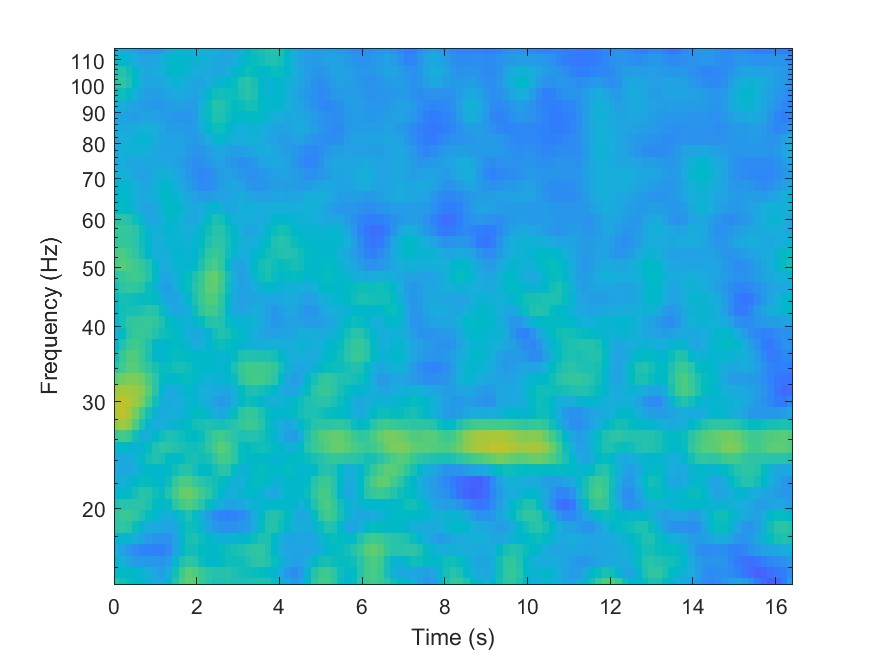
\includegraphics[width=\textwidth]{Bm_Ant-B_30.jpg}
                %                  \label{fig:BmA_ex}
                %              \end{subfigure}
                %              \hfill
                %              \begin{subfigure}[]{0.45\textwidth}
                %                      \centering
                %                      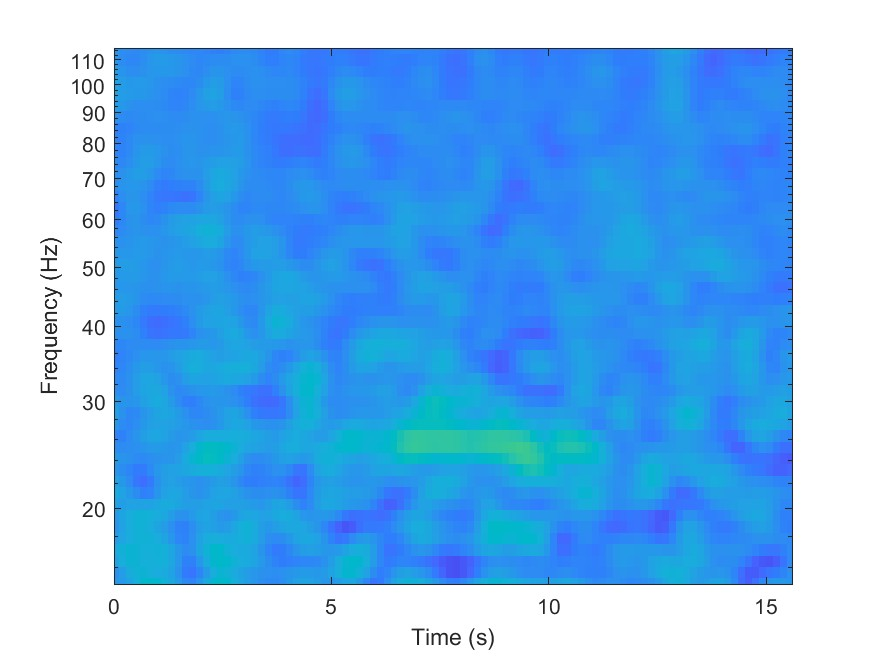
\includegraphics[width=\textwidth]{Bm_Ant-B_37.jpg}
                %                      \label{fig:BmB_ex}
                %                  \end{subfigure}
                %                  \hfill
                %                  \begin{subfigure}[]{0.45\textwidth}
                %                          \centering
                %                          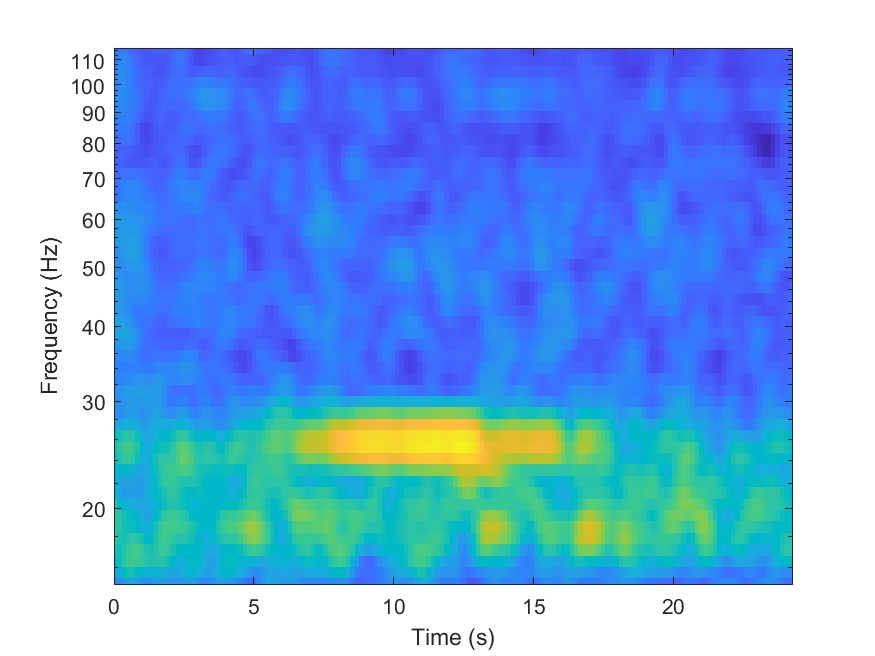
\includegraphics[width=\textwidth]{Bm_Ant-Z_27.jpg}
                %                          \label{fig:BmZ_ex}
                %                      \end{subfigure}
                %                      \hfill
                %                      \begin{subfigure}[]{0.45\textwidth}
                %                              \centering
                %                              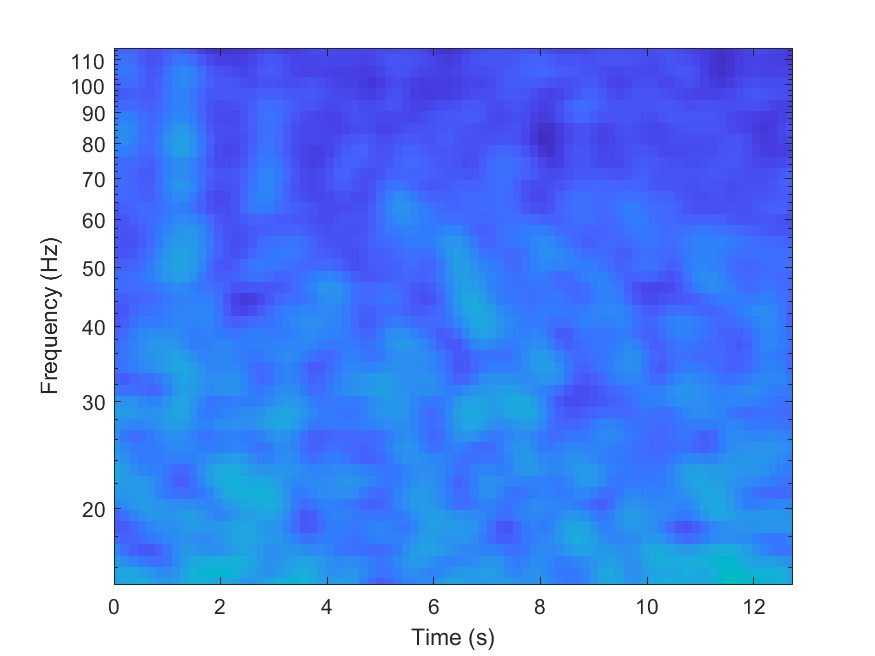
\includegraphics[width=\textwidth]{Bm_D_33.jpg}
                %                              \label{fig:BmD_ex}
                %                          \end{subfigure}
                %                             \caption{(a) \textit{Bm\_Ant\_A} labeled as \textit{Bm\_Ant\_B}, although the noise could be misinterpreted the ``tail" required for the B-type vocalisation. (b) Low SNR makes it difficult to distinguish between A-type and B-type calls. This example is labeled as \textit{Bm\_Ant\_B}. (c) A vocalisation more akin to the A-type may be easily mislabeled as \textit{Bm\_Ant\_Z} due to low-frequency noise. (d) The \textit{Bm\_D} class contains many low SNR annotations, some of which are likely patterns in the noise that have been misinterpreted as a vocalisation. Many of the misannotations in (a)-(d) become more apparent when using a constant Q transform such as the WST instead of a conventional \ac{stft}.}
                %                             \label{fig:Bm_misannotations}
                %                     \end{figure}
\end{subappendices}